% Магистерский диплом
% Воронежский государственный университет
%
% Выполнил: Кретов Павел Александрович, студент 6 курса физического факультета.
% Научный руководитель: Усков Григорий КОнстантинович, к.ф.-м.н.
% Июнь 2012 г.

\documentclass[a4paper,14pt,master]{disser}

\bibliographystyle{gost780u}
%\biboptions{compress}


\usepackage{mathtext}
%\usepackage{cmap}
% Русификация и utf-икация латеха
\usepackage[T2A]{fontenc}
\usepackage[utf8]{inputenc}
\usepackage[russian]{babel}

% Прочие пакеты и их настройки
\usepackage{amsmath}
\usepackage{amsfonts}
\usepackage{amssymb}
\usepackage{wasysym}  % for \oiint

\usepackage{graphicx}
\graphicspath{{../}}

\usepackage{verbatim}

\usepackage{tabularx}
\usepackage{multirow}

\usepackage{listings}
\lstloadlanguages{C++}
\lstset{language=C++,
        extendedchars=\true,
		basicstyle=\ttfamily\fontsize{11pt}{11pt}\selectfont}

\clubpenalty=10000
\widowpenalty=10000

\usepackage{geometry}
\geometry{
    left=2.5cm,
    right=1.5cm,
    top=1.5cm,
    bottom=1.0cm,
    footskip=1cm,
    includefoot}

\linespread{1.25}
%\onespacing
%\onehalfspacing



\parindent=1.1cm

\usepackage{url}

\setcounter{tocdepth}{1}

\usepackage{enumitem}
\newlist{where}{itemize}{1}
\newlist{chronology}{description}{1}
\setenumerate{
    leftmargin=\parindent,
    topsep=0cm,
    itemsep=0cm,
    parsep=0cm,
    partopsep=0cm}
\setitemize{
    label={--},
    leftmargin=\parindent,
    topsep=0cm,
    itemsep=0cm,
    parsep=0cm,
    partopsep=0cm}
\setdescription{
    topsep=0cm,
    leftmargin=\parindent,
    itemsep=0cm,
    parsep=0cm,
    partopsep=0cm}
\setlist[where]{
    label=,
    leftmargin=\parindent,
    topsep=0cm,
    itemsep=0cm,
    parsep=0cm,
    partopsep=0cm}
\setlist[chronology]{
    font=\normalfont,
    leftmargin=2.0cm,
    style=sameline,
    topsep=0.35cm,
    itemsep=0cm,
    parsep=0cm,
    partopsep=0cm}

%\renewcommand\chapter\addsectionw

%\usepackage{float}
%\newfloat{floatequation}{p}{floatequation.aux}{

\usepackage{calc}

\usepackage{numprint}

\usepackage{underscore}
\usepackage{listings}


\reversemarginpar


\allowdisplaybreaks

\renewcommand\epsilon\varepsilon
\renewcommand\phi\varphi
\renewcommand\le\leqslant
\renewcommand\ge\geqslant

\newcommand{\vect}[1]{\ensuremath{\vec{#1\mathstrut}}}

\makeatletter
%%%
\renewcommand\tocprethechapter{}
\renewcommand\tocpostthechapter{.}
\renewcommand\thechapteralign{}
\renewcommand\thechapterfont{\normalfont\bfseries}
\renewcommand\prethechapter{}
\renewcommand\postthechapter{.}
\renewcommand\tocchapterfont{\normalfont}
\renewcommand\tocchapterfillfont{\normalfont}
\renewcommand\tocchapternumfont{\normalfont}

%\renewcommand\chapterindent{}
\renewcommand\chapteralign{}
\renewcommand\chapterfont{\bfseries}
\renewcommand\beforechapter{}
\renewcommand\afterchapter{\par\nobreak\vskip 20\p@}

% Размер всех заголовков должен быть одинаковым.
\renewcommand\sectionfont{\normalfont\bfseries}

% Уберем дурацкие отступы после \paragraph и \subparagraрh.
\renewcommand\afterparagraph{-1ex}
\renewcommand\aftersubparagraph{-1ex}


\newcommand\tocchapterindent{0em}
\newcommand\tocchapternameindent{1.6em}

\renewcommand\tocposttheappendix{.}

%\renewcommand*\chapter{\clearpage\@startsection{chapter}{0}}
\renewcommand\l@chapter{\@tocline{chapter}{0}}

% Подписи к картинкам и таблицам должны быть того же размера, что
% и основной текст.
\renewcommand*\captionfont{\normalfont}
\renewcommand*\captionlabelfont{\normalfont}

\makeatother

%\DeclareMathOperator\div{div}
\DeclareMathOperator\rot{rot}
\DeclareMathOperator\grad{grad}

\newcommand{\VSWR}{\text{КСВН}}

\newcommand{\val}[1]{\numprint{#1}}
\newcommand{\valu}[2]{\val{#1}\,\ensuremath{#2}}

\newcommand\yee[3]{\left.#1\right|^{#2}_{#3}}
\newcommand\Yee[3]{#1\Big|^{#2}_{#3}}
\newcommand{\hanglimitsoperator}[4][c]{\text{\makebox[\widthof{$#2$}][#1]{ $#2^{#3}_{#4}$ }}}

\newcommand\fyee[3]{\hanglimitsoperator[l]{\left.#1\right|}{#2}{#3}~~~}
\newcommand\fYee[3]{\hanglimitsoperator[l]{#1\Big|}{#2}{#3}~~~}
\newcommand\yeediff[5]{\frac{\yee{#1}{#2}{#3} - \yee{#1}{#2}{#4}}{\Delta{#5}}}

\newcommand\code[1]{\texttt{#1}}

%\int\flimits^A_B
%\makebox[\widthof{\int}]\int\limits^A_B

% That special are only for convenience of browsing with xdvi program.
\special{papersize=\the\paperwidth,\the\paperheight}

% That special are only for convenience of browsing with xdvi program.
\special{papersize=\the\paperwidth,\the\paperheight}


\title{Метод конечных разностей во временной области}
\author{Кретов Павел Александрович}
\date{}

\begin{document}
    


\renewcommand*\contentsname{Оглавление}

\hyphenation{КСВН}

%%%

	%
%

\begin{titlepage}
\centering
%МИНОБРНАУКИ РОССИИ\\
%ФЕДЕРАЛЬНОЕ ГОСУДАРСТВЕННОЕ БЮДЖЕТНОЕ ОБРАЗОВАТЕЛЬНОЕ УЧРЕЖДЕНИЕ\\
%ВЫСШЕГО ПРОФЕССИОНАЛЬНОГО ОБРАЗОВАНИЯ\\
%<<ВОРОНЕЖСКИЙ ГОСУДАРСТВЕННЫЙ УНИВЕРСИТЕТ>>\\
Министерство образования и науки Российской Федерации\\
Федеральное государственное бюджетное образовательное учреждение\\
высшего профессионального образования\\
<<Воронежский государственный университет>>\\

\vspace{10mm}

%Факультет физический\\
Физический факультет\\
Кафедра электроники

\vspace{50mm}

\textbf{
    Исследование TEM-рупорных антенн для излучения и приема импульсных
    СШП-сигналов методом конечных разностей во~временной области}

\vspace{10mm}
Магистерская диссертация\\
\vspace{10mm}
011800 --- Радиофизика\\
Информационные системы и технологии\\
Информационные процессы и системы\\

\vspace{20mm}
\begin{tabularx}{\textwidth}{lll}
\multicolumn{3}{l}{Допущено к защите в ГАК} \\[5mm]
Зав.~кафедрой & \hspace{35mm} & Бобрешов\,А.\,М., д.\,ф.-м.\,н.,
\underline{\hspace{5mm}}.\underline{\hspace{5mm}}.\underline{\hspace{10mm}}~г.\\
Студент       & \hspace{35mm} & Кретов\,П.\,А.\\
Руководитель  & \hspace{35mm} & Усков\,Г.\,К., к.\,ф.-м.\,н.\\
\end{tabularx}

\vspace*{\fill}

Воронеж, 2012\,г.
\end{titlepage}
\setcounter{page}{2}

    
\noindent
{\newcolumntype{C}{>{\centering\arraybackslash}X}
\begin{tabularx}{\textwidth}{lCr}
УДК 621.396.67 & \textbf{Реферат} & Кретов\,П.\,А.
\end{tabularx}}
\vspace{10mm}

Расчет значений нижней граничной частоты для TEM-рупоров различной длины
с использованием метода конечных разностей во временной области.\\
Магистерская диссертация по направлению 010800 Радиофизика, Воронеж, ВГУ, 2012\,г.
--- \lastpage\,с., илл. 11, библ. 21 назв.

\vspace{10mm}

\noindent
\textbf{Ключевые слова:} сверхширокополосный сигнал, сверхкороткий импульс, TEM-рупорная антенна, граничная частота, метод конечных разностей, согласование волнового сопротивления, коэффициент стоячей волны по напряжению.

\vspace{10mm}
Рассматривалась задача моделирования TEM-рупорной антенны, нахождения коэффициента стоячей волны по напряжению на входе антенны. Проводились эксперименты по численному нахождению КСВН для антенн с различной геометрией. Для расчета использовался метод конечных разностей во временной области.
\newpage


	% --- kurswork-contents.tex ---

\tableofcontents



	%
%
%
\chapter* {Введение}
\addcontentsline {toc} {chapter} {Введение}

В~настоящее время все более актуальным становится исследование
сверхширокополосных радиосистем, использующих в качестве сигналов сверхкороткие
импульсы~(СКИ) субнаносекундной длительности. Среди антенн, пригодных для излучения
и приема СКИ сигналов, можно выделить ТЕМ-рупоры с переменным волновым
сопротивлением, которое на практике, как правило, изменяется от~\valu{50}{Ом}
в точке запитки до $120\pi$~Ом у раскрыва.

Анализу именно таких антенны посвящена данная работа. В ней дается описание
численных экспериментов по определению характеристик TEM-рупорных
антенн при излучении СКИ-сигналов с использованием метода конечных разностей
во~временной области (FDTD), описание принципов работы которого вместе
с основными дополнениями также приводится в работе.

Геометрия TEM-рупорных антенн сложна для аналитических вычислений, однако она
поддается анализу с помощью численных методов. Из существующих алгоритмов
численного решения уравнений Максвелла был выбран именно FDTD так, как он,
являясь временным методом (в отличие от частотных), позволяет:
\begin{itemize}
\item получить зависимости КСВН от частоты за один расчет с помощью быстрого
      преобразования Фурье от временных значений эквивалентного тока
      и напряжения;
\item получить форму сигнала в определенной точке пространства, что весьма
      полезно при анализе задач, связанных с~СКИ;
\item расчитать величину электромагнитного поля вне счетной области, что необходимо
      для нахождения диаграмм направленности.
\end{itemize}

Зависимость КСВН от частоты в рабочем диапазоне удобно использовать для оценки
уровня согласования антенны. При этом важным параметром для излучения СКИ
является нижняя граничная частота антенны, в качестве критерия для определения
которой можно принять требование не превышения КСВН во всем диапазоне частот
спектра излучаемого сигнала некоторого заранее выбранного значения.
Из теории плавных переходов известно, что
увеличение длины перехода с заданным профилем изменения волнового сопротивления
уменьшает его нижнюю граничную частоту перехода, поэтому в работе исследовалось
влияние длины ТЕМ-рупорной антенны с заданным экспоненциальным профилем
волнового сопротивления на КСВН и нижнюю граничную частоту антенны. С помощью
метода FDTD было проведено моделирование синтезированных профилей во временной
области, были построены и проанализированы зависимости КСВН от частоты
в диапазоне от \val{0.1}--\valu{10}{ГГц}.

Из-за большой ширины спектра СКИ-сигнала описание антенны
при помощи диаграмм направленности, используемых обычно в случае узкополосных
сигналов, не дает представления о форме и амплитуде СШП-импульса,
так как вид диаграммы направленности антенны
может кардинальным образом отличаться на разных частотах, входящих
в его спектр. Поэтому использование в этом случае
энергетических диаграмм направленности, выражающих полную энергию, пришедшуюся
на то или иное направление за все время излучения предпочтительнее.

Также в работе дается описание компьютерных программ, разработанных для того,
чтобы рассчитывать вышеописанные параметры во временной области методом FDTD.


	\chapter{Теоретическое введение}

	\section{Метод конечных разностей во временной области}
\label{section:CoreMethod}

\emph{Метод конечных разностей во временной области} (\emph{FDTD}) --- это
популярный численный метод моделирования электромагнитных полей. Он относительно
прост для понимания и реализации. Так как метод работает во временной области,
то он годится для решения задач в очень широком диапазоне частот.

Этот метод относится к общему классу сеточных методов решения дифференциальных
уравнений. В рамках этого метода уравнения Максвелла подвергаются дискретизации
с использованием центрально-разностной аппроксимации как по временной, так и по
пространственным координатам. Полученные конечно-разностные уравнения решаются
программными или аппаратными средствами в каждой точке временной сетки, причем,
компоненты вектора напряженности магнитного поля смещены на половину шага
дискретизации относительно компонент вектора напряженности электрического поля.
Расчет полей в ячейках сетки повторяется до тех пор, пока не будет получено
решение поставленной задачи в интересующем промежутке времени.


\subsection{Возникновение и развитие}

Базовый алгоритм метода был впервые предложен американским ученым Кейном Йе
(англ. Kane Yee) из Калифорнийского университета в~\cite{bib:Yee1966}. Однако,
само название «Finite-difference time-domain» и аббревиатура «FDTD» были даны
методу Алленом Тефлавом (англ. Allen Taflove) из Северо-западного университета
штата Иллинойс. Однако отсутствие мощных электронно-вычислительных машин привело
к тому, что
значительный импульс в развитии и применении метод получил лишь к началу 80-х.
В настоящее время метод FDTD интенсивно развивается, существует множество
дополнений к базовому алгоритму, значительно расширяющих область его приложений.
Некоторые из этих дополнений будут подробно описаны далее в работе.

\begin{chronology}

\item[1966~г.]
Йе разработал базовый алгоритм и вывел базовые уравнения~\cite{bib:Yee1966}.

\item[1975~г.]
Тефлав и Бродвин разработали критерии стабильности для алгоритма, разработанного
Йе. Были получены первые решения двумерных и трехмерных задач на взаимодействия
электромагнитной волны с веществом и первые биоэлектромагнитные
модели~\cite{bib:TafloveBrodwin1975}.

\item[1977~г.]
Холланд, Кунц и Ли применили алгоритм для решения
EMP-проблем~\cite{bib:KunzLee1978part1,bib:KunzLee1978part2}.

\item[1980~г.]
Тефлав ввел аббревиатуру FDTD и опубликовал первый проверенный расчетный
результат (моделировалось проникновение электромагнитных полей в металлическую
трехмерную полость)\cite{bib:Taflove1980}.

\item[1981~г.]
Мур опубликовал первое стабильное граничное условие поглощения второго
порядка~\cite{bib:Mur1981}.

\item[1984~г.]
Ляо разработал улучшенное условие поглощения, основанное на
пространственно-временной экстраполяции полей смежных с границей счетного
объема ячеек~\cite{bib:Liao1984}.
\end{chronology}

\noindent
Затем последовало множество работ, предлагающих усовершенствование метода.
Кроме того, важно понятие граничных условий на основе идеально сочетающихся
слоев (PML), которые были впервые разработаны в 1994~г. Жаном-Пьером
Беренже~\cite{bib:Berenger1994} для двумерного случая и были распространены
Кацем на трехмерный случай.

Примерно с 1990~г.\ метод конечных разностей стал основным для численного
решения многих научных и инженерных задач, связанных со взаимодействием
электромагнитных волн с веществом. Он может быть с успехом применен для решения
широкого спектра задач: от моделирования сверхдлинных электромагнитных волн
в~геофизике (включая процессы в ионосфере) и микроволн (например для изучения
сигнатурной радиолокации, расчета характеристик антенн, разработки беспроводных
устройств связи, в том числе цифровых) до решения задач в оптическом диапазоне
(фотонные кристаллы, наноплазмоника, солитоны и биофотоника). К 2006~г. число
публикаций, посвященных FDTD, достигло двух тысяч. В~настоящее
время 27 компаний разработали коммерческие программы, использующие метод
конечных разностей. Также существует 8~проектов с открытым исходными кодам
и 2~бесплатных с закрытым кодом, предназначенных только для некоммерческого
использования.
Более полный их список можно найти в~источнике~\cite{bib:WikipediaFdtdArticle}.


\subsection{Принципы работы}

Рассматривая уравнения Максвелла, легко заметить, что изменение электрического
поля во времени (частная производная по времени) зависит от изменения магнитного
поля в пространстве (ротора магнитного поля). Поэтому, в каждой точке
пространства значение вектора электрического поля в каждый момент времени
зависит от его значения в предыдущий момент времени и от изменения распределения
вектора напряженности магнитного поля в пространстве.

В то же время, из аналогичных рассуждений можно заключить, что значение
вектора~$\vect{H}$ в каждый момент времени зависит от его значения в предыдущий
момент времени и от изменения распределения вектора~$\vect{E}$ в пространстве.
В памяти компьютера хранятся значения векторов~$\vect{E}$ и~$\vect{H}$
в~каждой ячейке сетки, значения которых пересчитываются с каждой итерацией процесса по времени.

Написанное выше справедливо как для одномерного и двумерного случаев, так и для
трехмерного. Если задача поставлена в нескольких измерениях, то численный
расчет ротора полей сильно усложняется. Поэтому для упрощения расчетов в~методе
FDTD сетки электрического и магнитного поля сдвинуты друг относительно друга
так, что магнитное поле расчитывается в точках, расположенных ровно между
точками, в~которых расчитывается электрическое поле, и наоборот. Эта схема,
известная теперь под названием \emph{сетки Йе}, зарекомендовала себя как очень
надежная и в настоящее время составляет основу большинства современных
реализаций метода FDTD. Рисунок~\ref{fig:YeeCell} иллюстрирует вышесказанное.

Более того, Йе также предложил аналогичную схему для нахождения временных
производных: $\vect{E}$- и $\vect{H}$-компоненты сетки разделены во времени
половиной шага дискретизации.


\subsection{Использование}

Для использования метода необходимо задать счетную область.
\emph{Счетная область} (или \emph{счетный объем}) --- это та область
пространства, в пределах которой выполняется численное моделирование.
Счетным объемом также называется объем счетной области.

В каждой точке счетной области задается ее материал и вычисляются вектора
полей~$\vect{E}$ и~$\vect{H}$. Как правило, материал --- это вакуум (либо
воздух), металл или диэлектрик. Однако, возможно использование любой комбинации
диеэлектрической и магнитной проницаемости и удельной проводимости.

После того, как задана счетная область и материалы в ячейках сетки, необходимо
задать источники электромагнитных полей. В зависимости от задачи, источником
может быть точечным источником, плоской электромагнитной волной, полем витка
тока или чем-нибудь иным.

Так как вектора электрического и магнитного полей непосредственно определяются
в ходе моделирования, итоговым результатом, как правило, является серия значений
векторов полей в последовательные моменты времени в одной или нескольких точках
счетной области. Эти точки счетного объема называются \emph{пробниками}.

Полученные в результате моделирования векторы~$\vect{E}$ и~$\vect{H}$ могут быть
подвергнуты дополнительной обработке, которая, в том числе, может
происходить без остановки процесса моделирования и не мешает нахождению полей
в следующие моменты времени.

Так как по методу FDTD рассчитывается электромагнитное поле в ограниченной
пространственной области, излучаемые в пространство поля не могут быть рассчитаны
напрямую, но могут быть получены при помощи преобразований ближнего поля в дальнее.

\subsection{Достоинства и недостатки}

Любой численный метод имеет свои сильные и слабые стороны,
и метод FDTD не является исключением.

\subsubsection*{Достоинства:}
\begin{itemize}

\item
это очень разносторонний метод решения уравнений Максвелла, он
интуитивно понятен, поэтому пользователи могут легко разобраться в том, как он
работает и каких результатов ждать от его применения в той или иной задаче;

\item
работает во временной области, это значит, что за один этап моделирования
может быть получен результат в большом диапазоне частот, что может быть полезно,
например, при моделировании распространения широкополосных сигналов (например,
гауссовых импульсов) или при решении задач, для которых не известны резонансные
частоты;

\item
так как, согласно методу, поля вычисляются последовательно с течением времени,
это позволяет создавать анимированные изображения распространения волновых
процессов в счетном объеме, что может быть очень полезно для
понимания того, что происходит с моделью, и позволяют удостовериться, что модель
работает корректно;

\item
позволяет указать материал в каждой точке счетного объема и может быть
легко приспособлен для моделирования не только широкого спектра металлов и
диэлектриков, но и материалов с нелинейными свойствами;

\item
позволяет непосредственно моделировать эффекты на отверстиях, так же как
эффекты экранирования, причем поля внутри и вне экрана могут быть рассчитаны как
напрямую, так и косвенно;

\item
возвращает сразу значения векторов~$\vect{E}$ и~$\vect{H}$, что
очень удобно при решении большинства задач на электромагнитную совместимость
и электромагнитное взаимодействие, так как не требуется дополнительная обработка
результатов моделирования.
\end{itemize}
Кроме всего прочего, в пользу метода говорит то, что:
\begin{itemize}

\item
он является открытым и развивающимся, ему посвящено множество публикаций;

\item
возможна программная реализация метода, позволяющая неоднократно запускать
моделирование и использовать результаты, не прекращая работы, что может быть
полезно, например для оптимизации и синтеза формы сверхширокополосных антенн;

\item
программная реализация метода FDTD позволяет рассчитывать специфические для
приложений характеристики, такие как энергетические диаграммы направленности
антенн, и другие.
\end{itemize}

\subsubsection*{Недостатки:}
\begin{itemize}

\item
Весь счетный объем должен быть разбит на ячейки сеткой Йе, причем величина шага
дискретизации по пространству должна быть достаточно малой по сравнению
с наименьшей длиной волны, используемых в конкретной задаче. Кроме того, эта
величина ограничивает детализацию распределения материалов в пространстве.
Поэтому может оказаться, что счетный объем должен быть разделен на очень большое
число ячеек, что означает большие затраты памяти и большое время моделирования.
Наиболее сложно моделировать задачи с длинными, тонкими пространственными
структурами, например, поля проводников с током.

\item
FDTD рассчитывает поля в каждой точке счетного объема. Если требуется найти поле
на некотором отдалении от источника, скорее всего требуемый для этого счетный
объем окажется чрезмерно большим. Существуют расширения метода для нахождения
полей в дальней зоне, но они требуют дополнительной обработки результатов
моделирования.

\item
Так же это означает, что счетный объем должен быть конечным, чтобы уместиться
в памяти компьютера. В большинстве случаев это достигается с помощью задания
искусственных граничных условий. Но их нужно использовать с осторожностью,
чтобы свести к минимуму вызываемые ими искажения. В настоящее время известно
несколько эффективных граничных условий поглощения для алгоритма FDTD,
позволяющих имитировать бесконечную счетную область. Многие современные
реализации используют вместо них специальный абсорбирующий «материал»,
называемый \emph{идеально согласованным слоем} (англ. \emph{Perfectly Matched
Layer}).
\end{itemize}


\subsection{Базовые уравнения}

Как уже было сказано, метод FDTD предполагает введение сетки, которая на
практике представляет собой обыкновенный трехмерный массив, в котором хранятся
векторы полей и пространственная структура. Расчет заключается в том, что
программа просматривает по очереди все элементы этого массива, в порядке
возрастания индексов, перевычисляя его элементы по приведенным ниже формулам.

Для компонентов магнитного поля:
\label{eq:BaseFdtdEquations}
\begin{align*}
	\Yee{H_x}{n+1/2}{i,j,k} &=
        \Yee{H_x}{n-1/2}{i,j,k} - \frac{\Delta{t}}{\mu}
        \left[
            \frac{\yee{E_z}{n}{i,j+1,k} - \yee{E_z}{n}{i,j,k}}{\Delta{y}} -
            \frac{\yee{E_y}{n}{i,j,k+1} - \yee{E_y}{n}{i,j,k}}{\Delta{z}}
        \right], \\
	\Yee{H_y}{n+1/2}{i,j,k} &=
        \Yee{H_y}{n-1/2}{i,j,k} - \frac{\Delta{t}}{\mu}
        \left[
            \frac{\yee{E_x}{n}{i,j,k+1} - \yee{E_x}{n}{i,j,k}}{\Delta{z}} -
            \frac{\yee{E_z}{n}{i+1,j,k} - \yee{E_z}{n}{i,j,k}}{\Delta{x}}
        \right], \\
	\Yee{H_z}{n+1/2}{i,j,k} &=
        \Yee{H_z}{n-1/2}{i,j,k} - \frac{\Delta{t}}{\mu}
        \left[
            \frac{\yee{E_y}{n}{i+1,j,k} - \yee{E_y}{n}{i,j,k}}{\Delta{x}} -
            \frac{\yee{E_x}{n}{i,j+1,k} - \yee{E_x}{n}{i,j,k}}{\Delta{y}}
        \right],
\end{align*}

Для компонентов электрического поля:
\begin{align*}
	\fYee{E_x}{n+1}{i,j,k} &=
        \frac{1-\frac{\sigma\Delta{t}}{2\epsilon}}
             {1+\frac{\sigma\Delta{t}}{2\epsilon}} \fYee{E_x}{n}{i,j,k} +
        \frac{\frac{\Delta{t}}{\epsilon}}
             {1+\frac{\sigma\Delta{t}}{2\epsilon}}
        \left[
            \frac{\yee{H_z}{n+1/2}{i,j,k} - \yee{H_z}{n+1/2}{i,j-1,k}}{\Delta{y}} -
            \frac{\yee{H_y}{n+1/2}{i,j,k} - \yee{H_y}{n+1/2}{i,j,k-1}}{\Delta{z}}
        \right], \\
	\fYee{E_y}{n+1}{i,j,k} &=
        \frac{1-\frac{\sigma\Delta{t}}{2\epsilon}}
	         {1+\frac{\sigma\Delta{t}}{2\epsilon}} \fYee{E_y}{n}{i,j,k} +
        \frac{\frac{\Delta{t}}{\epsilon}}
             {1+\frac{\sigma\Delta{t}}{2\epsilon}}
        \left[
            \frac{\yee{H_x}{n+1/2}{i,j,k} - \yee{H_x}{n+1/2}{i,j,k-1}}{\Delta{z}} -
            \frac{\yee{H_z}{n+1/2}{i,j,k} - \yee{H_z}{n+1/2}{i-1,j,k}}{\Delta{x}}
        \right], \\
	\fYee{E_z}{n+1}{i,j,k} &=
        \frac{1-\frac{\sigma\Delta{t}}{2\epsilon}}
             {1+\frac{\sigma\Delta{t}}{2\epsilon}} \fYee{E_z}{n}{i,j,k} +
        \frac{\frac{\Delta{t}}{\epsilon}}
             {1+\frac{\sigma\Delta{t}}{2\epsilon}}
        \left[
            \frac{\yee{H_y}{n+1/2}{i,j,k} - \yee{H_y}{n+1/2}{i-1,j,k}}{\Delta{x}} -
            \frac{\yee{H_x}{n+1/2}{i,j,k} - \yee{H_x}{n+1/2}{i,j-1,k}}{\Delta{y}}
        \right].
\end{align*}

\noindent
Тут приведены формулы, позволяющие вычислить каждую из компонент векторов
напряженности электрического и магнитного полей. В этих формулах используются
следующие обозначения:
%%
\begin{where}
\item $\sigma$ --- удельная проводимость материала в данной ячейке сетки;
\item $\varepsilon$ --- абсолютная диэлектрическая проницаемость материала;
\item $\mu$ --- абсолютная магнитная проницаемость материала;
\item $\Delta t$ --- шаг дискретизации по временной координате;
\item $\Delta x$, $\Delta y$, $\Delta z$ --- шаги дискретизации
      по пространственным осям.
\end{where}

\noindent
Необходимо заметить, что величина $\Delta t$ определяет частотные характеристики
метода: наивысшая частота в спектре сигналов, распространение которых
моделируется, не должна превышать~$f_{\text{max}} = 1/\Delta{t}$.

В записи формул мы использовали вертикальную черту и дополнительные индексы у компонент векторов
напряженности для того, чтобы показать, к какому шагу по времени и ячейке пространственной сетки они относятся.
Так, например, запись $\yee{H_x}{n+1/2}{i,j,k}$ означает, что перед нами
$x$-компонента вектора $\vect{H}$, взятая в ячейке $(i, j, k)$ сетки Йе
в момент времени $n+1/2$. Здесь время измеряется в шагах
дискретизации~$\Delta{t}$, а так как компоненты вектора~$\vect{H}$ смещены на
полшага во времени относительно компонент вектора~$\vect{E}$, им соответствуют
полуцелые индексы. (В программных реализациях полуцелые индексы увеличивают на
одну вторую, так как большинство языков программирования не поддерживают
работу с массивами, индексы которых не являются целыми числами.)

Необходимо заметить, что пересчет значений компонент выполняется «на месте», то
есть рассчитанное в каждый последующий момент времени значение помещается в ту
же ячейку сетки Йе, в которой находилось значение в предыдущий момент. Это
позволяет несколько снизить требования к оперативной памяти, предъявляемые методом.


\subsection{Вывод базовых уравнений}

Базовые уравнения метода, приведенные в предыдущем пункте работы, получаются
путем применения к системе вихревых уравнений Максвелла явной конечно-разностной
схемы второго порядка.

Итак, пусть в каждой точке пространства задана диэлектрическая
проницаемость~$\epsilon(\vect{r})$, магнитная проницаемость~$\mu(\vect{r})$
и удельная проводимость~$\sigma(\vect{r})$. Тогда мы можем записать уравнения
Максвелла для векторов~$\vect{E}$, $\vect{D}$, $\vect{H}$ и~$\vect{B}$ обычным
образом:
%%
\begin{equation}
    \label{eq:MaxwellEquations}
    \left\{
    \begin{aligned}
        \rot{\vect{E}(\vect{r},t)} &=
            -\mu(\vect{r})\frac{\partial\vect{H}(\vect{r},t)}{\partial t}
            -\sigma^*(\vect{r})H(\vect{r},t), \\
        \rot{\vect{H}}(\vect{r},t) &=
            \epsilon{\vect{r}}\frac{\partial\vect{E}(\vect{r},t)}{\partial t} +
            \sigma(\vect{r})E(\vect{r},t).
    \end{aligned}
    \right.
\end{equation}

Подвергнем эту систему явной конечно-разностной дискретизации по формуле:
\vspace{-0.3cm}
\begin{equation}
    \label{eq:FiniteDifferenceScheme}
    f'(\xi) =
        \frac{f(\xi+\frac{\Delta\xi}{2})-f(\xi-\frac{\Delta\xi}{2})}{\Delta\xi}
        + O(\Delta\xi^2) \approx
        \frac{f(\xi+\frac{\Delta\xi}{2})-f(\xi-\frac{\Delta\xi}{2})}{\Delta\xi},
\end{equation}
%%
где $f$ --- любая из компонент векторов напряженности,
    $\xi$ --- любая из пространственно-временных координат $(x,y,z,t)$.

Йе предложил такой способ дискретизации, при котором электрические и магнитные
поля смещаются друг относительно друга на половину шага, как в пространстве,
так и по времени. При этом между ячейками автоматически выполняются граничные
условия. Расположение полей в элементе объема сетки Йе показано на
рис.~\ref{fig:YeeCell}.

Такой подход к дискретизации системы дифференциальных уравнений
Максвелла~\eqref{eq:MaxwellEquations} позволяет получить простую систему
конечно-разностных уравнений. Для этого запишем выражение для роторов
в декартовой системе координат и произведем замену всех производных по
формуле~\eqref{eq:FiniteDifferenceScheme}. Упростив полученные выражения,
получим формулы на стр.~\pageref{eq:BaseFdtdEquations}, выведенные Йе.

Эта система уравнений решается итеративно, что является преимуществом метода
FDTD. Алгоритм является устойчивым при выполнении приведенного ниже условия
Куранта, связывающего шаги дискретизации по пространству и времени:
%%
\begin{equation}
\label{eq:CourantCondition}
\frac{1}{\Delta t^2} \ge c^2
\left(
    \frac{1}{\Delta x^2} +
    \frac{1}{\Delta y^2} +
    \frac{1}{\Delta z^2}
\right),
\end{equation}
%%
где $c$ --- скорость света в вакууме.

% --- Yee-cube.svg: 440x310 pixel, 72dpi, 15.52x10.94 cm, bb=0 0 440 310 ---
\begin{figure}[p]
\centering
%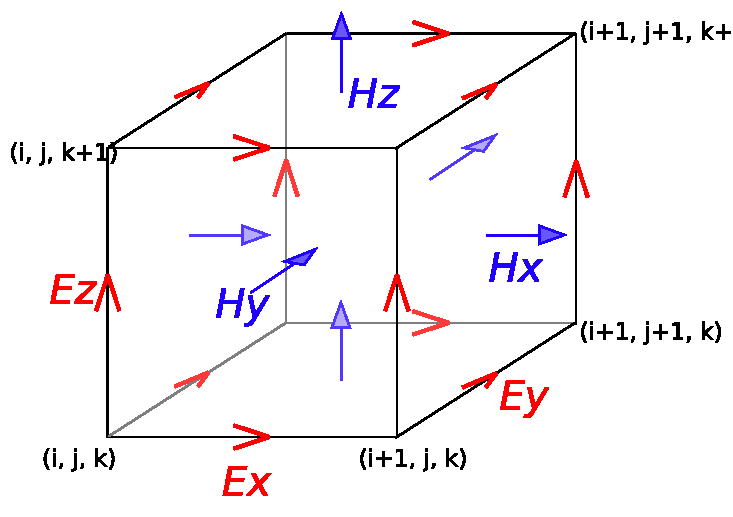
\includegraphics[width=75mm]{graphics/yee-cell}
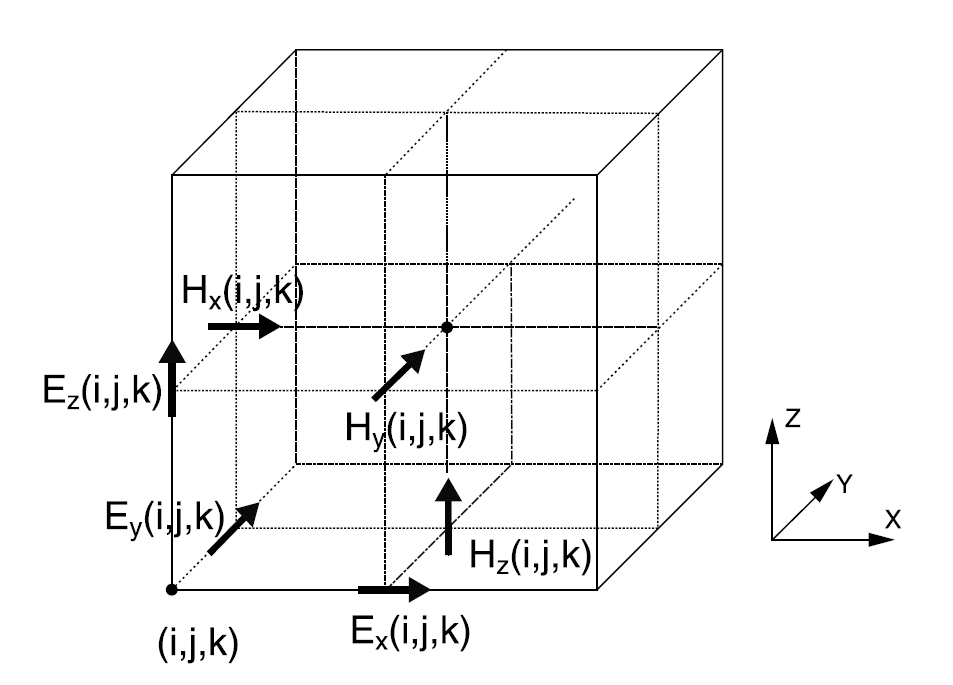
\includegraphics[width=0.5\textwidth]{graphics/Yee-Cubes}
\caption{Поля в ячейке сетки Йе.
    Из таких ячеек составляется пространственная трехмерная сетка Йе, взаимодействие
    волн с веществом учитывается заданием в каждой ячейке значений диэлектрической
    и магнитной проницаемости и удельной проводимости.}
\label{fig:YeeCell}
\end{figure}

	

\section{Решение задач на открытых областях}
\label{section:GridReduction}

Приведенные здесь базовый алгоритм в неизменном виде пригоден только в случае
бесконечной счетной области. Очевидно, этот случай невозможно осуществить на
практике (по крайней мере, за конечное время). Поэтому были разработаны методы,
позволяющие получать решение, близкое к теоретическому, при ограниченном счетном
объеме. Это возможно благодаря дополнительной обработке полей на границе
счетного объема.


\subsection{Методы сокращения сетки}

В настоящее время наиболее широко используемые методы ограничения счетной
области. Основными такими методами являются:
\begin{itemize}
    \item граничное условие отражения;
	\item граничные условия поглощения;
	\item системы идеально согласованных слоев (PML).
\end{itemize}

Использование первого из этих методов приводит к многократному переотражению
сигнала внутри счетной области, два других позволяют уменьшить отражение волны
от границы. Условия поглощения намного проще, чем PML, однако, система
согласованных слоев позволяет получить на порядки меньшие по величине
коэффициенты отражения от границы.

Понятие идеально согласованных слоев (PML) было введено Жаном-Пьером Беренже
в~\cite{bib:Berenger1994}. Позже оригинальная методика Беренже была
усовершенствована и дополнена, в результате были разработаны методы
UPML (uniaxial PML), CPML (convolutional PML), а также PML высших порядков.
Два последних метода имеют повышенную способность к поглощению падающих волн
и принципиально могут быть помещены ближе к изучаемой рассеивающей или
излучающей структуре, чем оригинальные PML Беренже.

В данной работе ниже мы подробно рассмотрим условия PML и определим их основные
характеристики.


\subsection{Условие идеального отражения}

Предположим, что за счетным объемом напряженность поля равна нулю. Это означало
бы, что счетный объем окружен бесконечным идеальным проводником, а значит, все
волны полностью отразятся назад внутрь счетного объема. Хотя в природе не
существует идеальных проводников, это условие может быть полезным в ряде
случаев.

Так как волны отражаются внутрь счетного объема, это значит, что он --- счетный
объем --- должен быть достаточно большим, чтобы границы находились достаточно
далеко от рассчитываемой структуры и отраженная от границ волна не успевала
существенно повлиять на физические процессы. Однако, это приводит к серьезному
увеличению времени расчета и объема необходимой для моделирования памяти.

На практике это условие реализуется очень просто: счетный объем окружается
дополнительным слоем ячеек, поле в которых никогда не высчитывается и изначально
инициализируется нулями.


\subsection{Условия поглощения}

Наличие отражения волн внутрь счетного объема в большинстве случаев искажает
картину распространения сигнала. С этим можно бороться при помощи специальных
граничных условий, которые поглощали бы падающие волны, не давая им отразиться
от границы объема.

Условия поглощения (англ.~absorbtion conditions, ABC) были разработаны для
моделирования границы счетного объема, поглощающей падающие на нее волны. Все
эти условия используют значения полей в смежных ячейках и в предыдущие моменты
времени для того, чтобы получить текущее значение поля на границе.

Всего известно достаточно много граничных условий поглощения, однако некоторые
из них не могут быть применены в прямоугольных декартовых координатах, другие
требуют для работы слишком громоздких вычислений. Поэтому реально применяются
граничные условия только двух типов: граничные условия Ляо и Мура. Так как на
практике эти граничные условия применяются намного реже, чем PML, в данной
работе они не будут рассматриваться.


\subsection{Граничные условия PML}

Данный тип граничных условий (строго говоря, являющихся поглощающей приграничной
областью, а не граничным условием, как таковым) обладает одними из лучших
характеристик. При использовании PML предполагается, что счетную область
окружается слоем анизотропного поглощающего материала, обладающий рядом свойств,
подробно описанных ниже.

\paragraph*{Волновое сопротивление.}
На границе раздела «счетная область --- согласованный слой» волновое
сопротивление не изменяется, что достигается выполнением следующего соотношения:
%%
\begin{equation}
\label{eq:EpsilonAndMu}
\frac{\sigma}{\varepsilon} = \frac{\sigma^*}{\mu}.
\end{equation}

\paragraph*{Профиль потерь.}
Электрическая и магнитная проводимость возрастают с увеличением расстояния
вглубь слоя PML по некоторому закону, называемому \emph{профилем потерь}.

В оригинальной работе Беренже был предложен следующий профиль потерь, как
оптимальный по уровню отражения от границы
раздела~\cite{bib:Berenger1994,bib:Berenger1996}:
%%
\begin{itemize}

\item для электрической проводимости:
\begin{align}
\label{eq:LossProfile}
\sigma_\text{PML}(i) &= \left\{
\begin{array}{ll}
    \sigma_\text{PML0}\frac{\sqrt{g}-1}{\ln{g}}     & \text{при~} i=0,\\
    \sigma_\text{PML0}\frac{g-1}{\sqrt{g}\ln{g}}g^i & \text{при~} i=\frac12,1,\frac32,~\ldots
\end{array}
\right.\\
\sigma_\text{PML0} &= -\frac{\epsilon_0 \ln{g}} {2 d \epsilon_0\mu_0 (g^N-1)} \ln{r};
% NOTE: Здесь применена особая уличная магия.
\intertext{\item для магнитной проводимости:}
%\begin{align}
    \sigma^{*}_\text{PML}(i) &= \frac{\mu}{\epsilon} \sigma_\text{PML}(i).
\end{align}

\end{itemize}

\noindent
В приведенной выше формуле фигурируют следующие величины:
\begin{where}
\item $g$ --- параметр, подбираемый эмпирически;
\item $r$ --- требуемый коэффициент отражения;
\item $d$ --- интервал дискретизации пространства в данном направлении;
\item $N$ --- толщина слоя PML.
\end{where}

\noindent
Приблизительная оценка толщины слоя PML может быть получена из следующего
соотношения:
\begin{equation}
\label{eq:hz1}
    N_\text{min}= \frac{1}{\ln g}
    \left[
        1 - \frac{\Theta t_p(\sqrt{g}-1)}{4\pi d \sqrt{\epsilon_0\mu_0}} \ln{r}
    \right],
\end{equation}
где $t_p$ --- длительность процесса моделирования во времени,
а параметр~$\Theta$ подбираются эмпирически (обычно $\Theta\approx10$).

\paragraph*{Частота отсечки.}
При использовании системы идеально согласованных слоев область допустимых частот
становится ограниченной снизу. Сигналы с частотой, меньшей чем некоторое
значение $f_{min}$ (называемое \emph{частотой отсечки}), отражаются от границы
PML. Ниже приведено выражение для частоты отсечки:
\begin{equation}
    \label{eq:PmlCutoffFrequency}
    f_{min} = \frac{\sigma_\text{PML}(0)}{2\pi\epsilon_0}.
\end{equation}


\subsection{Базовые уравнения PML}

Основная идея получения базовых уравнений для расчета компонентов поля
в согласованном слое состоит в том, что компоненты векторов $\vect{E}$
и $\vect{H}$ представляются в виде суммы двух слагаемых:
\begin{equation}
\label{eq:PmlSplitFieldEquations}
\left\{
    \begin{aligned}
        E_x = E_{xy}+E_{xz}, \\
        E_y = E_{yx}+E_{yz}, \\
        E_z = E_{zx}+E_{zy}.
    \end{aligned}
\right.\quad
\left\{
    \begin{aligned}
        H_x = H_{xy}+H_{xz}, \\
        H_y = H_{yx}+H_{yz}, \\
        H_z = H_{zx}+H_{zy}.
    \end{aligned}
\right.
\end{equation}

% TODO: Доверстать этот пиздец.
% \begin{пиздец}

\begin{eqnarray}
\label{eq:pml13}
%---
\left\{
\begin{array}{rcl}
  %--- xy
  \varepsilon \frac{\partial}{\partial t}E_{xy} + \sigma_y E_{xy} & = & \frac{\partial}{\partial y}(H_{zx}+H_{zy}) \\
  %--- xz
  \varepsilon \frac{\partial}{\partial t}E_{xz} + \sigma_z E_{xz} & = & \frac{\partial}{\partial z}(H_{yz}+H_{yx}) \\
  %--- yz
  \varepsilon \frac{\partial}{\partial t}E_{yz} + \sigma_z E_{yz} & = & \frac{\partial}{\partial z}(H_{xy}+H_{xz}) \\
  %--- yx
  \varepsilon \frac{\partial}{\partial t}E_{yx} + \sigma_x E_{yx} & = & \frac{\partial}{\partial x}(H_{zx}+H_{zy}) \\
  %--- zx
  \varepsilon \frac{\partial}{\partial t}E_{zx} + \sigma_x E_{zx} & = & \frac{\partial}{\partial x}(H_{yx}+H_{yz}) \\
  %--- zy
  \varepsilon \frac{\partial}{\partial t}E_{zy} + \sigma_y E_{zy} & = & \frac{\partial}{\partial y}(H_{xy}+H_{xz}) \\
\end{array}
\right.
  \\ %-------------------------------
\left\{
\begin{array}{rcl}
  %--- xy
  \varepsilon \frac{\partial}{\partial t}H_{xy} + \sigma_y^* H_{xy} & = & \frac{\partial}{\partial y}(E_{zx}+E_{zy}) \\
  %--- xz
  \varepsilon \frac{\partial}{\partial t}H_{xz} + \sigma_z^* H_{xz} & = & \frac{\partial}{\partial z}(E_{yz}+E_{yx}) \\
  %--- yz
  \varepsilon \frac{\partial}{\partial t}H_{yz} + \sigma_z^* H_{yz} & = & \frac{\partial}{\partial z}(E_{xy}+E_{xz}) \\
  %--- yx
  \varepsilon \frac{\partial}{\partial t}H_{yx} + \sigma_x^* H_{yx} & = & \frac{\partial}{\partial x}(E_{zx}+E_{zy}) \\
  %--- zx
  \varepsilon \frac{\partial}{\partial t}H_{zx} + \sigma_x^* H_{zx} & = & \frac{\partial}{\partial x}(E_{yx}+E_{yz}) \\
  %--- zy
  \varepsilon \frac{\partial}{\partial t}H_{zy} + \sigma_y^* H_{zy} & = & \frac{\partial}{\partial y}(E_{xy}+E_{xz}) \\
\end{array}
\right.
\end{eqnarray}

Анизотропия согласованного слоя проявляется в следующем: каждой ячейке соответствует набор $(\sigma_x,\sigma_y,\sigma_z)$, причем элемент $\sigma_\alpha$ ($\alpha={x,y,z}$) не равен нулю только для ячеек слоя, пересекаемого соответствующей осью координат.


В дискретной форме уравнения (\ref{eq:pml13}) выглядят следующим образом:
\begin{equation}
\left\{
\begin{aligned}
H_{xy (i,j,k)}^{n+1} = D_{ay (i,j,k)} H_{xy (i,j,k)}^{n} - D_{by (i,j,k)}
\left[
    \frac{E_{z (i,j+1,k)}^n - E_{z (i,j,k)}^n}{\Delta y}
\right] \\
%---
H_{xz (i,j,k)}^{n+1} = D_{az (i,j,k)} H_{xz (i,j,k)}^{n} - D_{bz (i,j,k)}
\left[
    \frac{E_{y (i,j,k+1)}^n - E_{y (i,j,k)}^n}{\Delta z}
\right] \\
%---
H_{yx (i,j,k)}^{n+1} = D_{ax (i,j,k)} H_{yx (i,j,k)}^{n} - D_{bx (i,j,k)}
\left[
    \frac{E_{z (i+1,j,k)}^n - E_{z (i,j,k)}^n}{\Delta x}
\right] \\
%---
H_{yz (i,j,k)}^{n+1} = D_{az (i,j,k)} H_{yz (i,j,k)}^{n} - D_{bz (i,j,k)}
\left[
    \frac{E_{x (i,j,k+1)}^n - E_{x (i,j,k)}^n}{\Delta z}
\right] \\
%---
H_{zx (i,j,k)}^{n+1} = D_{ax (i,j,k)} H_{zx (i,j,k)}^{n} - D_{bx (i,j,k)}
\left[
    \frac{E_{y (i+1,j,k)}^n - E_{z (i,j,k)}^n}{\Delta x}
\right] \\
%---
H_{zy (i,j,k)}^{n+1} = D_{ay (i,j,k)} H_{zy (i,j,k)}^{n} - D_{by (i,j,k)}
\left[
    \frac{E_{x (i,j+1,k)}^n - E_{x (i,j,k)}^n}{\Delta y}
\right]
\end{aligned}
\right.
\end{equation}

\begin{equation}
\left\{
\begin{aligned}
E_{xy (i,j,k)}^{n+1} = C_{ay (i,j,k)} E_{xy (i,j,k)}^{n} - C_{by (i,j,k)}
\left[
    \frac{H_{z (i,j,k)}^{n+1} - H_{z (i,j-1,k)}^{n+1}}{\Delta y}
\right] \\
%---
E_{xz (i,j,k)}^{n+1} = C_{az (i,j,k)} E_{xz (i,j,k)}^{n} - C_{bz (i,j,k)}
\left[
    \frac{H_{y (i,j,k)}^{n+1} - H_{y (i,j,k-1)}^{n+1}}{\Delta z}
\right] \\
%---
E_{yx (i,j,k)}^{n+1} = C_{ax (i,j,k)} E_{yx (i,j,k)}^{n} - C_{bx (i,j,k)}
\left[
    \frac{H_{z (i,j,k)}^{n+1} - H_{z (i-1,j,k)}^{n+1}}{\Delta x}
\right] \\
%---
E_{yz (i,j,k)}^{n+1} = C_{az (i,j,k)} E_{yz (i,j,k)}^{n} - C_{bz (i,j,k)}
\left[
    \frac{H_{x (i,j,k)}^{n+1} - H_{x (i,j,k-1)}^{n+1}}{\Delta z}
\right] \\
%---
E_{zx (i,j,k)}^{n+1} = C_{ax (i,j,k)} E_{zx (i,j,k)}^{n} - C_{bx (i,j,k)}
\left[
    \frac{H_{y (i,j,k)}^{n+1} - H_{z (i-1,j,k)}^{n+1}}{\Delta x}
\right] \\
%---
E_{zy (i,j,k)}^{n+1} = C_{ay (i,j,k)} E_{zy (i,j,k)}^{n} - C_{by (i,j,k)}
\left[
    \frac{H_{x (i,j,k)}^{n+1} - H_{x (i,j-1,k)}^{n+1}}{\Delta y}
\right]
\end{aligned}
\right.
\end{equation}

Коэффициенты $C$ и $D$ находятся по формулам:
\begin{equation*}
\begin{aligned}
D_{ax (i,j,k)} =
\frac
{
    1-\frac{\sigma_{x (i,j,k)}^*\Delta t}{2\mu_{(i,j,k)}}
}{
    1+\frac{\sigma_{x (i,j,k)}^*\Delta t}{2\mu_{(i,j,k)}}
}, \\
%---
D_{bx (i,j,k)} =
\frac
{
    \frac{\Delta t}{\mu_{(i,j,k)}}
}{
    1+\frac{\sigma_{x (i,j,k)}^*\Delta t}{2\mu_{(i,j,k)}}
},
\end{aligned}
%---------------
\quad
\begin{aligned}
D_{ay (i,j,k)} =
\frac
{
    1-\frac{\sigma_{y (i,j,k)}^*\Delta t}{2\mu_{(i,j,k)}}
}{
    1+\frac{\sigma_{y (i,j,k)}^*\Delta t}{2\mu_{(i,j,k)}}
}, \\
%---
D_{by (i,j,k)} =
\frac
{
    \frac{\Delta t}{\mu_{(i,j,k)}}
}{
    1+\frac{\sigma_{y (i,j,k)}^*\Delta t}{2\mu_{(i,j,k)}}
},
\end{aligned}
%---------------
\quad
\begin{aligned}
D_{az (i,j,k)} =
\frac
{
    1-\frac{\sigma_{z (i,j,k)}^*\Delta t}{2\mu_{(i,j,k)}}
}{
    1+\frac{\sigma_{z (i,j,k)}^*\Delta t}{2\mu_{(i,j,k)}}
}, \\
%---
D_{bz (i,j,k)} =
\frac
{
    \frac{\Delta t}{\mu_{(i,j,k)}}
}{
    1+\frac{\sigma_{z (i,j,k)}^*\Delta t}{2\mu_{(i,j,k)}}
},
\end{aligned}
%---------------
\end{equation*}

\begin{equation*}
\begin{aligned}
D_{ax (i,j,k)} =
\frac
{
    1-\frac{\sigma_{x (i,j,k)}\Delta t}{2\mu_{(i,j,k)}}
}{
    1+\frac{\sigma_{x (i,j,k)}\Delta t}{2\mu_{(i,j,k)}}
}, \\
%---
D_{bx (i,j,k)} =
\frac
{
    \frac{\Delta t}{\mu_{(i,j,k)}}
}{
    1+\frac{\sigma_{x (i,j,k)}\Delta t}{2\mu_{(i,j,k)}}
},
\end{aligned}
%---------------
\quad
\begin{aligned}
D_{ay (i,j,k)} =
\frac
{
    1-\frac{\sigma_{y (i,j,k)}\Delta t}{2\mu_{(i,j,k)}}
}{
    1+\frac{\sigma_{y (i,j,k)}\Delta t}{2\mu_{(i,j,k)}}
}, \\
%---
D_{by (i,j,k)} =
\frac
{
    \frac{\Delta t}{\mu_{(i,j,k)}}
}{
    1+\frac{\sigma_{y (i,j,k)}\Delta t}{2\mu_{(i,j,k)}}
},
\end{aligned}
%---------------
\quad
\begin{aligned}
D_{az (i,j,k)} =
\frac
{
    1-\frac{\sigma_{z (i,j,k)}\Delta t}{2\mu_{(i,j,k)}}
}{
    1+\frac{\sigma_{z (i,j,k)}\Delta t}{2\mu_{(i,j,k)}}
}, \\
%---
D_{bz (i,j,k)} =
\frac
{
    \frac{\Delta t}{\mu_{(i,j,k)}}
}{
    1+\frac{\sigma_{z (i,j,k)}\Delta t}{2\mu_{(i,j,k)}}
},
\end{aligned}
%---------------
\end{equation*}

% \end{пиздец}

Следует заметить, что в реальной ситуации всегда присутствуют
отражения~\cite{bib:Berenger1994,bib:Berenger1996}.
Они складываются из:
\begin{itemize}
  \item отражений от первого слоя PML;
  \item отражений между слоями PML;
  \item отражений от проводящей границы за последним слоем PML.
\end{itemize}

\noindent
В связи с этим, для уменьшения отражения от первого слоя значение~$\sigma_0$
специально выбирается небольшим. Отражения между слоями подавляются за счет
ограничения скорости роста профиля потерь. Для уменьшения влияния волны,
отраженной от бесконечно проводящей границы, увеличивается число слоев
PML~\cite{bib:Berenger1996}.

	%
%
%

\section{Точечный резистивный источник напряжения}
\label{div:LumpedSource}

Возможность моделировать сосредоточенные элементы вводится как расширение
основного метода~\cite{bib:Taflove1995,bib:Davidson2005,bib:PiketMay1994,
bib:Maloney1994}. При этом границы применения метода существенно расширяются.
В частности, точечный генератор напряжения с заданным внутренним сопротивлением
оказывается весьма удобным для моделирования источников питания.

Достоинством этого дополнения является то, что при его использовании вид базовых
уравнений меняется весьма незначительно. Например,если источник ориентирован
вдоль оси~$z$, то в системе уравнений Макселла~\eqref{eq:MaxwellEquations}
изменится только одна составляющая векторного уравнения для ротора~$\vect{H}$:
\begin{equation}
    \label{eq:LumpedSource:MaxwellEquationsAmendment}
    (\rot\vect{H})_z = \epsilon\frac{\partial{E_z}}{\partial{t}} +
        \sigma E_z + \frac{I_L}{\Delta{x}\Delta{y}},
\end{equation}
где $I_L$ --- ток через источник.

Подвернув уравнение~\eqref{eq:LumpedSource:MaxwellEquationsAmendment} действию
разностной схемы~\eqref{eq:FiniteDifferenceScheme} и полагая~$\sigma=0$ получим
следующую формулу:
\begin{multline}
    \label{eq:LumpedSource:FdtdEquationsAmendmentWithI}
    \fYee{E_z}{n+1}{i,j,k} = \fYee{E_z}{n}{i,j,k} +
        \frac{\Delta{t}}{\yee{\epsilon}{}{i,j,k}}
        \left[
            \frac{\yee{H_y}{n+1}{i,j,k}-\yee{H_y}{n+1}{i-1,j,k}}{\Delta{x}} -
            \frac{\yee{H_x}{n+1}{i,j,k}-\yee{H_x}{n+1}{i,j-1,k}}{\Delta{y}}
        \right] - \\ -
        \frac{\yee{I_L}{n+1}{}\Delta{t}}
             {\yee{\epsilon}{}{i,j,k}\Delta{x}\Delta{y}}.
\end{multline}

Согласно закону Ома, для рассматриваемого сосредоточенного генератора напряжения
с внутренним сопротивлением $R$ будет иметь место равенство
\begin{equation}
    \label{eq:LumpedSource:OhmLaw}
    \fYee{I_L}{n+1}{} = \frac{\Delta{z}}{2R}
    \left(
        \fYee{E_z}{n+1}{i,j,k} - \Yee{E_z}{n}{i,j,k}
    \right) +
    \frac{\yee{V_s}{n+1}{}}{R},
\end{equation}
где $V_s$ --- генерируемое источником напряжение.

После подстановки~\eqref{eq:LumpedSource:OhmLaw}
в~\eqref{eq:LumpedSource:FdtdEquationsAmendmentWithI} получим простое уравнение
для~$E_z$:
\begin{multline}
    \label{eq:LumpedSource:FdtdEquationsAmendmentWithU}
    \fYee{E_z}{n+1}{i,j,k} =
        \fYee{C_E}{}{i,j,k}\fYee{E_z}{n}{i,j,k}~~+~~
        \Yee{C_H}{}{i,j,k}
        \left[
            \frac{\yee{H_y}{n+1}{i,j,k}-\yee{H_y}{n+1}{i-1,j,k}}{\Delta{x}}
        \right. - \\ -
        \left.
            \frac{\yee{H_x}{n+1}{i,j,k}-\yee{H_x}{n+1}{i,j-1,k}}{\Delta{y}} +
            \frac{\yee{V_s}{n+1}{}}{R\Delta{x}\Delta{y}}
        \right],
\end{multline}
где $C_E$ и~$C_H$ определяются по формулам:
\begin{equation}
    \newcommand\XA{\displaystyle
        \frac{\Delta{t}}{\yee{\epsilon}{}{i,j,k}}}
    \newcommand\XB{\displaystyle
        \frac{\Delta{t}\Delta{z}}{2R\yee{\epsilon}{}{i,j,k}\Delta{x}\Delta{y}}}
    % --
    \fYee{C_E}{}{i,j,k} = \frac{1-\XB}{1+\XB}, \quad
    \fYee{C_H}{}{i,j,k} = \frac{\XA}{1+\XB}.
\end{equation}

    %
%
%
\section{Задание источников поля с помощью метода~TF/SF}

В рамках метода FDTD принципиально возможны два способа задания источника поля:
\begin{itemize}
\item источник находится внутри счетного объема;
\item источник находится вне счетного объема.
\end{itemize}
Примером первого типа источника может быть, скажем, сосредоточенный резистивный
источник напряжения, рассмотренный в разделе~\ref{div:LumpedSource}. Источники
второго типа представляют собой фронт волны, падающей на счетную область. Для
задания такого источника удобно использовать
\emph{метод TF/SF}~\cite{bib:Taflove1995,bib:Davidson2005,bib:Berenger1994,
bib:Berenger1996}, или \emph{метод разделения области моделирования на область
общего поля и область рассеянного поля} (англ. total field и scattered field).
Пример разбиения расчетной области для двумерного случая приведен на
рис.~\ref{fig:Tfsf:SubdivisionExample}.

Область общего поля выбирается так, чтобы в ней полностью находился рассеивающий
объект (которым может быть и излучающая антенна), вся оставшаяся часть --- это
область рассеянного поля. В области рассеянного поля рассматривается только
рассеянное поле, а в области общего --- и рассеянное и падающее. На границе
между этими областями устанавливаются специальные граничные условия. Их суть
заключается в том, что поле вне TF/SF-границы не должно содержать падающей
составляющей --- она вычитается с соответствующими коэффициентами для
компонентов~$\vect{H}$ и~$\vect{E}$ из выражений для полей граничных с внешней
стороны ячеек~\cite{bib:Bogolyubov2006}. При моделирования распространения
падающей составляющей решается вспомогательная одномерная задача, рассмотренная
ниже.

Выражения для~$H$ и~$E$ компонент поля в приграничных по отношению к области
TF/SF ячейках для случая TEM-волны, распространяющейся вдоль оси $x$
($\vect{H}=\{H_x;0;0\}$, $\vect{E}=\{0;0;E_z\}$), можно увидеть на
стр.~\pageref{eq:Tfsf:BasicEquationsOnSeparatePage}, так как они слишком
громоздки для того, чтобы приводить их полностью в тексте работы.

% --- Термоядерный пиздец на отдельной странице.
\begin{figure}[p]
\label{eq:Tfsf:BasicEquationsOnSeparatePage}

\newcommand\Imin{I_\text{min}}
\newcommand\Imax{I_\text{max}}
\newcommand\Jmin{J_\text{min}}
\newcommand\Jmax{J_\text{max}}
\newcommand\Kmin{K_\text{min}}
\newcommand\Kmax{K_\text{max}}
\newlength\separator
\setlength\separator{5mm}
\begin{multline}
    \label{eq:Tfsf:MainEquations}
    % --
    \begin{aligned}
    \fYee{H_x}{n+1}{i,j,k} =
        \fYee{D_E}{}{i,j,k} \fYee{H_x}{n}{i,j,k} +
        \Yee{D_H}{}{i,j,k}
        \left[
            \yeediff{E_y}{n}{i,j,k+1}{i,j,k}{z} -
            \yeediff{E_z}{n}{i,j+1,k}{i,j,k}{y}
        \right. - \\ -
        \left.
            \delta_{j,\Jmin-1}\frac{\yee{E_s}{n}{i,\Jmin,k}}{\Delta{y}} +
            \delta_{j,\Jmax}\frac{\yee{E_s}{n}{i,\Jmax+1,k}}{\Delta{y}}
        \right],
    \end{aligned}\\[\separator]
    \begin{aligned}
    \fYee{H_y}{n+1}{i,j,k} =
        \fYee{D_E}{}{i,j,k} \fYee{H_y}{n}{i,j,k} +
        \Yee{D_H}{}{i,j,k}
        \left[
            \yeediff{E_z}{n}{i+1,j,k}{i,j,k}{x} -
            \yeediff{E_x}{n}{i,j,k+1}{i,j,k}{z}
        \right. - \\ -
        \left.
            \delta_{i,\Imin-1}\frac{\yee{E_s}{n}{\Imin,j,k}}{\Delta{x}} +
            \delta_{i,\Imax}\frac{\yee{E_s}{n}{\Imax+1,j,k}}{\Delta{x}}
        \right],
    \end{aligned}\\[\separator]
    \begin{aligned}
    \fYee{H_z}{n+1}{i,j,k} =
        \fYee{D_E}{}{i,j,k} \fYee{H_z}{n}{i,j,k} +
        \Yee{D_H}{}{i,j,k}
        \left[
            \yeediff{E_x}{n}{i,j+1,k}{i,j,k}{y} -
            \yeediff{E_y}{n}{i+1,j,k}{i,j,k}{x}
        \right],
    \end{aligned}\\[\separator]
    \begin{aligned}
    \fYee{E_x}{n+1}{i,j,k} =
        \fYee{C_E}{}{i,j,k} \fYee{E_x}{n}{i,j,k} +
        \Yee{C_H}{}{i,j,k}
        \left[
            \yeediff{H_z}{n+1}{i,j,k}{i,j-1,k}{y} -
            \yeediff{H_y}{n+1}{i,j,k}{i,k,k-1}{z}
        \right. + \\ +
        \left.
            \delta_{k,\Kmax+1}\frac{\yee{H_s}{n+1}{i,j,\Kmax}}{\Delta{z}} -
            \delta_{k,\Kmin}\frac{\yee{H_s}{n+1}{i,j,\Kmin-1}}{\Delta{z}}
        \right],
    \end{aligned}\\[\separator]
    \begin{aligned}
    \fYee{E_y}{n+1}{i,j,k} =
        \fYee{C_E}{}{i,j,k} \fYee{E_y}{n}{i,j,k} +
        \Yee{C_H}{}{i,j,k}
        \left[
            \yeediff{H_x}{n+1}{i,j,k}{i,j,k-1}{z} -
            \yeediff{H_z}{n+1}{i,j,k}{i-1,k,k}{x}
        \right],
    \end{aligned}\\[\separator]
    \begin{aligned}
    \fYee{E_z}{n+1}{i,j,k} =
        \fYee{C_E}{}{i,j,k} \fYee{E_z}{n}{i,j,k} +
        \Yee{C_H}{}{i,j,k}
        \left[
            \yeediff{H_y}{n+1}{i,j,k}{i-1,j,k}{x} -
            \yeediff{H_x}{n+1}{i,j,k}{i,k-1,k}{y}
        \right. + \\ +
        \left.
            \delta_{i,\Imax+1}\frac{\yee{H_s}{n+1}{\Imax,j,k}}{\Delta{x}} -
            \delta_{i,\Imin}\frac{\yee{H_s}{n+1}{\Imin-1,j,k}}{\Delta{x}}
        \right].
    \end{aligned}
\end{multline}

Формулы для моделировании с помощью метода TF/SF, падающая волна направлена
сверху вниз вдоль оси~$Oz$. Здесь $\delta_{i,j}$ --- символ Кронекера,
$I_\text{min}$, $I_\text{max}$, $J_\text{min}$, $J_\text{max}$, $K_\text{min}$,
$K_\text{max}$ --- индексы границы TF/SF области в массиве ячеек.
%Коэффициенты~$C_E$, $C_H$, $D_E$ и $D_H$ вычисляются согласно
%формулам~\eqref{eq:Tfsf:MainEquationsCoefficients}.
\end{figure}

% --- Продолжение громадных формул на всю страницу.
% TODO: Набрать эти ужасные формулы и добавить на них ссылки.
\begin{figure}
    \begin{align*}
    \end{align*}
\end{figure}

%% --
\begin{figure}
\centering
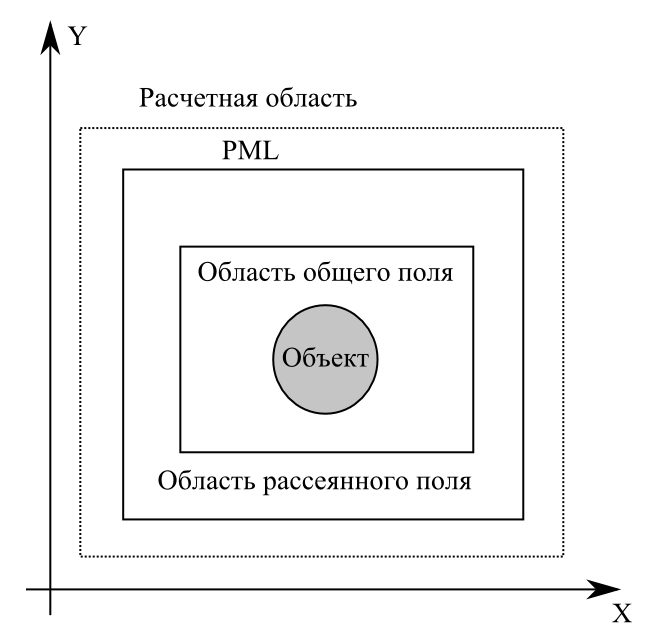
\includegraphics[width=0.5\textwidth]{graphics/tfsf-subdivision-example}
\caption{Пример разбиения расчетной области.}
\label{fig:Tfsf:SubdivisionExample}
\end{figure}

    
\section{Программные средства для моделирования}

Для проведения численных экспериментов было необходимо соответствующее
программное обеспечение. Несмотря на то, что существует значительное количество
программ для моделирования электродинамических задач при помощи метода FDTD,
было решено использовать собственную реализацию, так как доступные открытые
аналоги не устраивали по качеству исполнения, а проприетарные --- тем, что
их рабочие алгоритмы закрыты.

Итак, для моделирования TEM-рупорных антенн, описанного в последующих разделах,
ипользовалась связка из нескольких компьютерных программ, разработанных на
кафедре электроники физического факультета ВГУ. Схема их взаимодействия
представлена на рис.~\ref{fig:Programs:WorkFlow}.

% --- Рисунок
\begin{figure}[p]
\centering
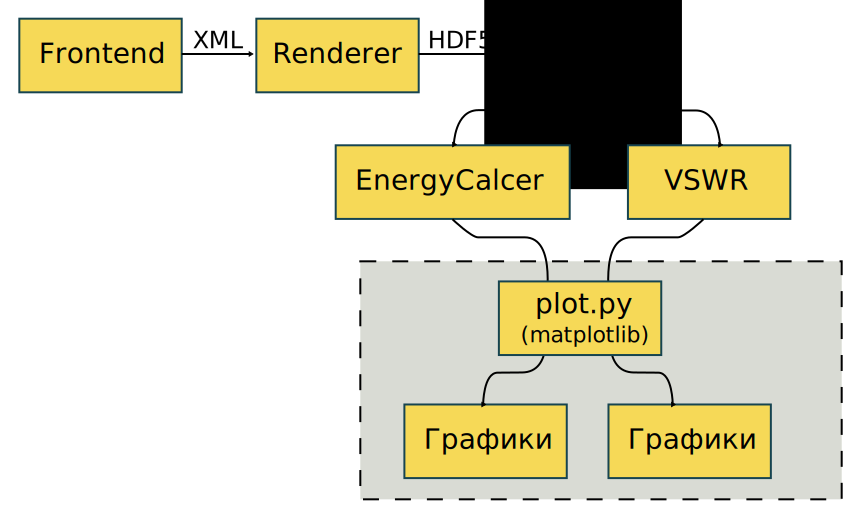
\includegraphics[width=0.7\textwidth]{graphics/programs-work-flow}
\caption{Взаимодействие компонентов программного комплекса моделирования.}
\label{fig:Programs:WorkFlow}
\end{figure}

Функциональное назначение отдельных блоков следующее:
\begin{itemize}
\item Frontend --- редактор трехмерной структуры, подлежащей анализу;
\item Renderer --- формирует трехмерную сетку счетной области, преобразовывая
      структуру из XML-представления, которое является рабочим фоматом
      предыдущей программы, в бинарное представление на основе формата HDF~5,
      удобное для проведения моделирования;
\item Fdtd3d --- расчетный модуль, выполняющий непосредственно моделирование
      и нахождение полей в дальней зоне;
\item EnergyCalcer --- расчитывает энергетические диаграммы направленности,
      используя рассчитанные предыдущей программой поля в дальней зоне;
\item VSWR --- расчитывает коэффициент стоячей волны по напряжению по
      результатам моделирования, полученным программой Fdtd3d;
\item plot.py --- скрипт на языке Python, строящий графики для наглядного
      представления результатов моделирования.
\end{itemize}

Пример работы программы Fdtd Frontend представлен на
рисунках~\ref{fig:Programs:LinearScreenshot}
и~\ref{fig:Programs:ExponentialScreenshot}, полученная в результате
преобразования сетка изображена на
рисунках~\ref{fig:Programs:RenderedLinearScreenshot}
и~\ref{fig:Programs:RenderedLinearScreenshot}. В пункте~\ref{div:FileFormat}
приводится описание бинарного формата данных, связывающего пользовательский
программный модуль с расчетным.

% --- Русонок.
\begin{figure}[p]
\centering
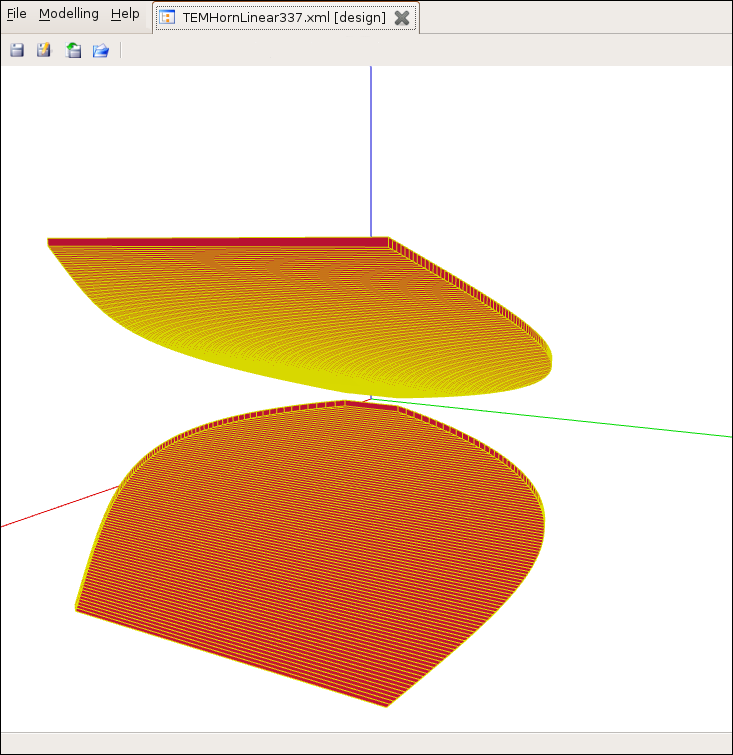
\includegraphics[width=\textwidth]{graphics/screenshot-tem-horn-linear-377}
\caption{
    Пример рабочего окна программы Fdtd Frontend с загруженной антенной
    с линейным профилем раскрыва и выходным волновым
    сопротивлением~$Z_R=\valu{377}{Ом}$.}
\label{fig:Programs:LinearScreenshot}
\end{figure}

% --- Русонок.
\begin{figure}[p]
\centering
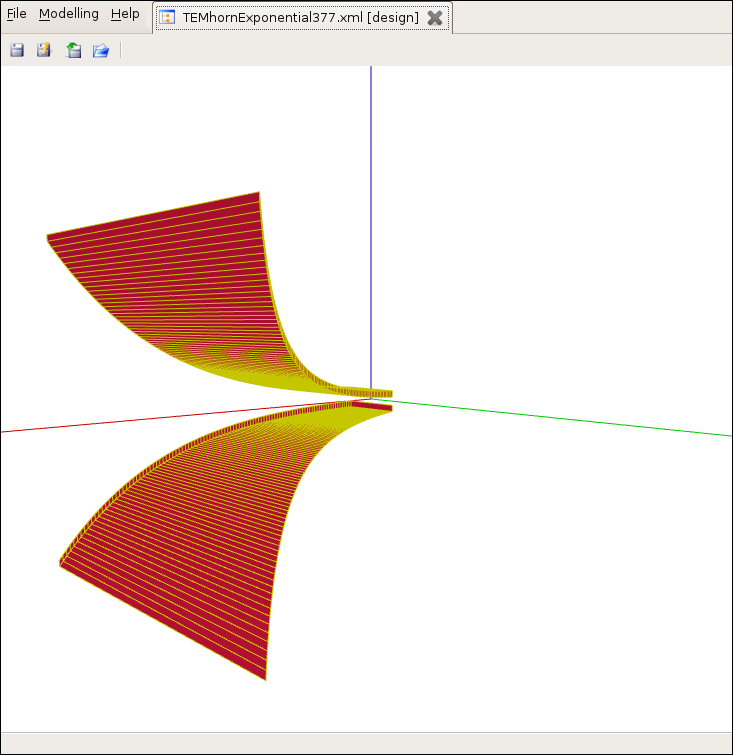
\includegraphics[width=\textwidth]{graphics/screenshot-tem-horn-exponential-377}
\caption{
    Пример рабочего окна программы Fdtd Frontend с загруженной антенной
    с экспоненциальным профилем раскрыва и выходным волновым
    сопротивлением~$Z_R=\valu{377}{Ом}$.}
\label{fig:Programs:ExponentialScreenshot}
\end{figure}

% --- Русонок.
\begin{figure}[p]
\centering
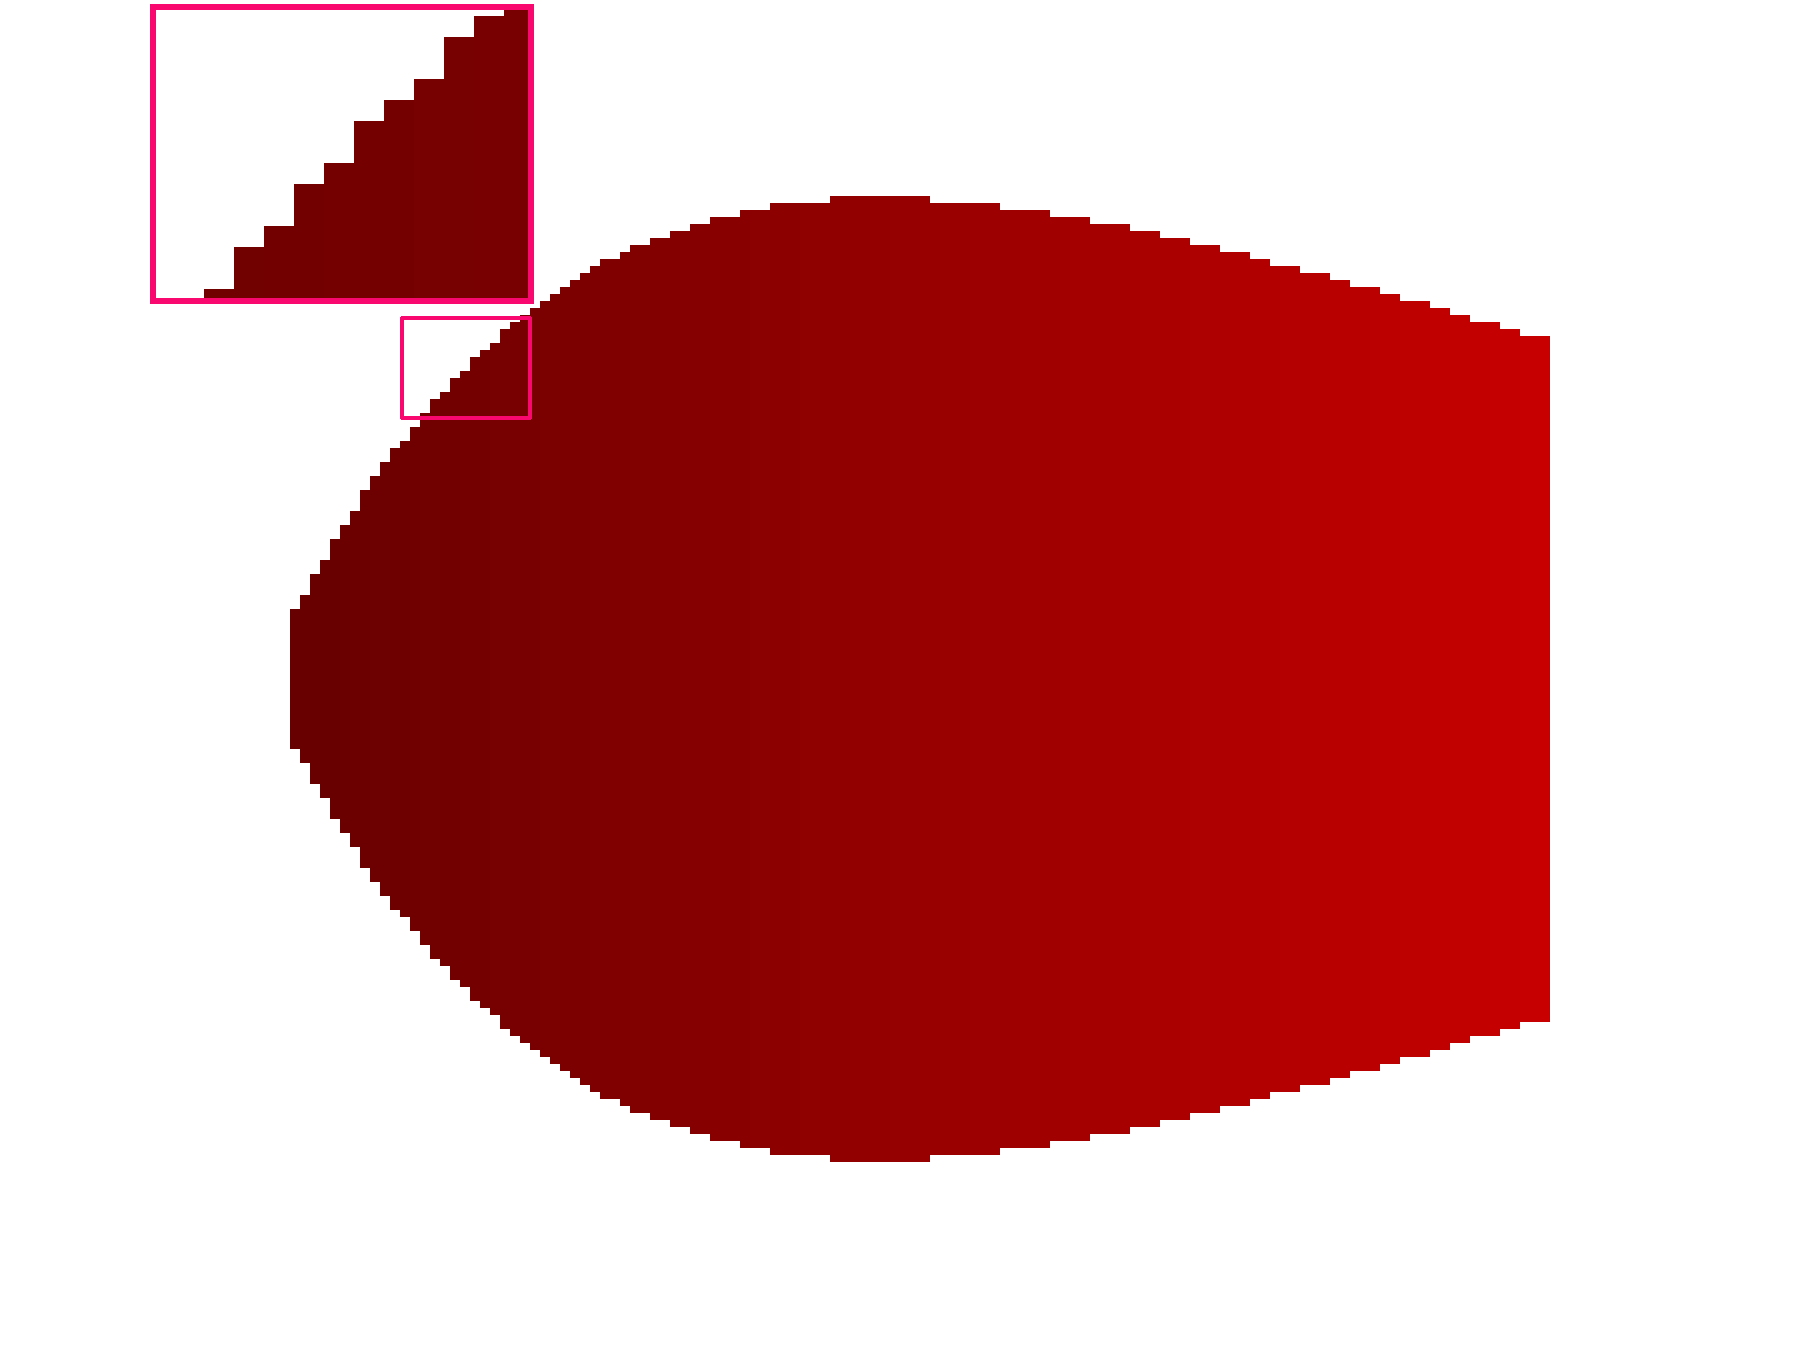
\includegraphics[width=\textwidth]{graphics/screenshot-rendered-linear-377}
\caption{
    Расчетная сетка антенны с линейным профилем раскрыва и выходным волновым
    сопротивлением~$Z_R=\valu{377}{Ом}$, вид сверху.}
\label{fig:Programs:RenderedLinearScreenshot}
\end{figure}

% --- Русонок.
\begin{figure}[p]
\centering
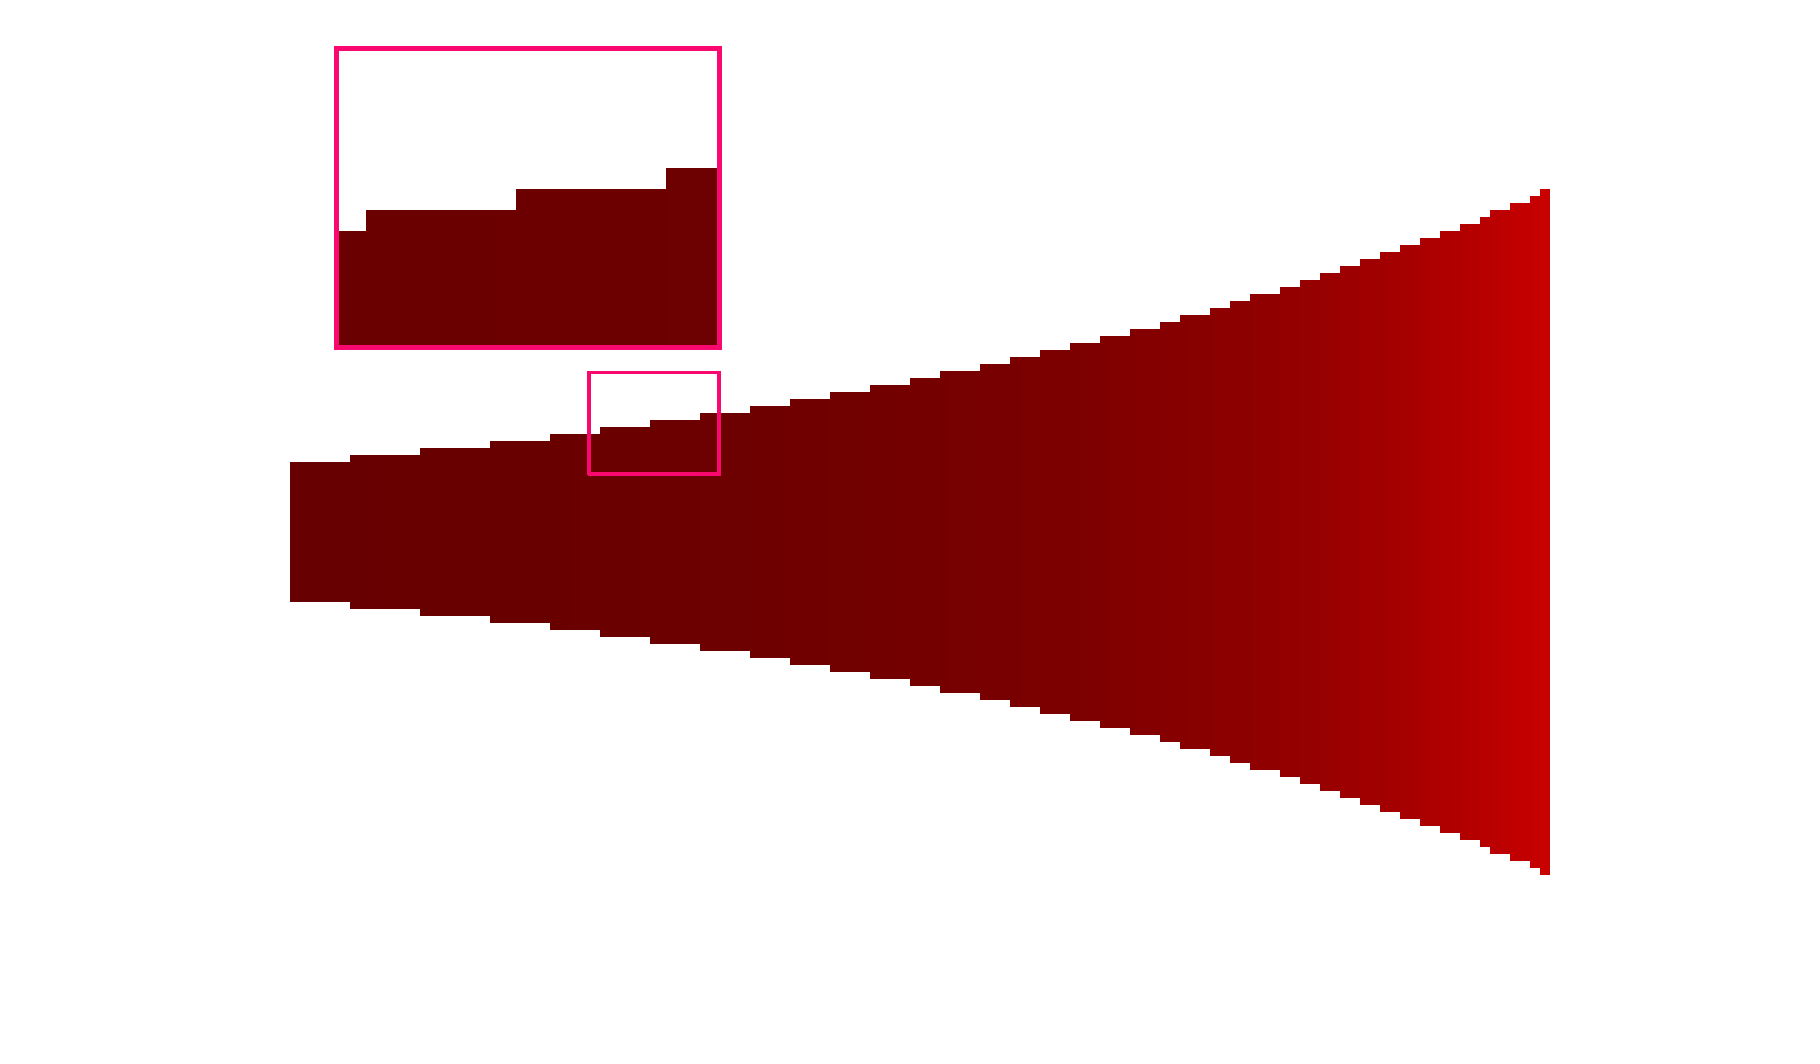
\includegraphics[width=\textwidth]{graphics/screenshot-rendered-exponential-377}
\caption{
    Расчетная сетка антенны с линейным профилем раскрыва и выходным волновым
    сопротивлением~$Z_R=\valu{377}{Ом}$, вид сверху.}
\label{fig:Programs:RenderedExponentialScreenshot}
\end{figure}

    
\section{Описание формата представления расчетной задачи}
\label{div:FileFormat}

\subsection{Введение}

В ходе работы над графическим интерфейсом к программе Fdtd3d, неоднократно
рассматриваемой нами в предыдущих работах, остро возникла необходимость
в создании (и стандартизации) некоторого формата файлов, который мог бы
использоваться для обмена данными между программой-редактором и программой,
непосредственно выполняющей численное моделирование задачи, сформулированной
пользователем в интерактивном режиме. Данные, в передаче которых возникла
необходимость, включают в себя информацию~о:
\begin{itemize}
\item дискретизации счетных пространства и времени;
\item используемых на границах счетного объема граничных условиях;
\item области TFSF;
\item области вычисления интеграла Кирхгофа для расчета полей в дальней зоне;
\item свойствах используемых в задаче материалах;
\item распределении этих материалов в дискретном пространстве;
\item расположении в счетном объеме пробников;
\item расположении в счетном объеме сосредоточенных элементов.
\end{itemize}

Помимо перечисленных данных приветствуется поддержка форматом дополнительной
информации определенного рода (метаданных), такой как:
\begin{itemize}
\item номер версии формата, с помощью которого был создан файл;
\item название и версия приложения, записавшего файл;
\item дата и время создания файла;
\item дата и время последней модификации файла;
\item имя пользователя, создавшего данный файл;
\item название организации, имеющей отношение к информации, записанной в файле.
\end{itemize}
Более подробно назначение каждого поля будет расписано в пункте работы,
посвященном детальному описанию структуры формата.

К формату данных предъявлялся следующий список требований:
\begin{itemize}
\item поддержка больших объёмов данных (как минимум порядка нескольких
      гигабайт);
\item высокая производительность операций чтения и записи;
\item расширяемость формата с сохранением совместимости;
\item возможность использования в параллельных программах (в перспективе);
\item возможность поточной передачи данных по сети (в перспективе);
\item поддержка прозрачного механизма компрессии/декомпрессии данных «на лету»
      (в перспективе).
\end{itemize}

Так как обеспечить выполнение всех этих требований представляется работой
в высшей степени нетривиальной и трудоемкой, было решено отказаться от попыток
создания собственного формата данных «с нуля», а вместо этого найти готовое
решение, по возможности --- распространяемое на условиях какой-либо свободной
лицензии. Такое решение было найдено и о нем пойдет речь в следующей части
работы.


\subsection{О формате HDF~5}

Аббревиатура HDF расшифровывается как Hierarchical Data Format, что можно
перевести на русский язык как <<иерархический формат данных>>. Цифра~<<5>>
относится к версии формата --- пятой, на данный момент последней и наиболее
совершенной в технологическом плане (однако по-прежнему поддерживается
предыдущая версия формата --- HDF~4, т.~к. файлы, записанные в этом формате,
все еще используются в работе некоторых организаций). Первые версии формата
были разработаны Национальным центром по применению
суперкомпьютеров~\cite{bib:NcsaWebsite} (университет штата Иллинойс, США) в конце
1980-x годов, в 2004~г. была основана некоммерческая организация HDF~Group~\cite{bib:HdfGroupWebsite},
призванная координировать развитие формата. В настоящее время этой организацией
разработана библиотека для встраивания поддержки формата в пользовательские
приложения, а также набор прикладных программ для работы с файлами форматов
HDF~4/HDF~5.

HDF~Group официально поддерживает API к библиотеке HDF~5 для следующих языков
программирования: C, C++, Fortran~77/90, Java. Кроме того, существуют сторонние
проекты, адаптирующие библиотеку для использования в программах на: Perl,
Python, GDL, IDL, языках математических пакетов MATLAB, Scilab и Mathematica.
Формат широко используется многими компаниями в исследовательской работе
в различных областях науки, для примера достаточно упомянуть такие известные
организации, как NASA и Intel. Более полный список проектов, использующих HDF~5,
можно найти по адресу~[3]
Однако, вернемся к списку требований, перечисленных в первом разделе. В ходе
исследования официальной документации было выяснено, что формат HDF~5
удовлетворят всем этим требованиями. А именно:
\begin{itemize}
\item
поддерживаются очень большие объемы данных, в отличие от четвертой версии
формата, где размер файла был ограничен \valu{2}{ГБ} из-за использования
32-битных знаковых целых чисел для адресации;

\item
иерархичность формата и использование символьных имен позволяет добиться
совместимости между версиями как в прямом, так и в обратном направлении;

\item
имеется встроенная поддержка параллельных программ, написанных с использованием
MPI, использующая функции MPI~I/O из MPI~2;

\item
поддерживается работа с сетевыми потоками;

\item
имеется возможность прозрачного сжатия данных про помощи т.~н. \emph{фильтров}.
\end{itemize}

Также отметим, что используемая HDF лицензия является свободной
и не ограничивает распространение и использование (в том числе коммерческое)
ни оригинальных, ни модифицированных исходных кодов библиотеки при условии
сохранения упоминания оригинальных авторов и явного указания на факт модификации
исходного кода. С полным текстом оригинальной лицензии на английском языке можно
ознакомиться на сайте HDF~Group~\cite{bib:HdfGroupWebsite}.


\subsection{Базовые понятия HDF~5}

Рассмотрим основные понятия, с которыми мы неизбежно сталкиваемся при работе
с файлами в формате HDF5. Это типы данных, пространства данных, наборы данных
и группы. Ниже мы объясним их назначение (в скобках приведено оригинальное
англоязычное название, используемое в документации проекта HDF).

\emph{Тип данных} (\emph{datatype}) определяет формат единичного элемента
данных некоторого вида. Типы данных могут быть как \emph{элементарными}
(\emph{atomic}), представленные, например, целыми числами и числами с плавающей
запятой, единичными символами и строками символов, так и \emph{составными}
(\emph{compound}), включающими в себя данные разных типов.

\emph{Пространство данных} (\emph{dataspace}) определяет способ организации
множества однотипных элементов, не зависящий от конкретного типа. Согласно
документации, пространства могут быть \emph{простыми} (\emph{simple})
и \emph{сложными} (\emph{complex}), однако реализация сложных пространств данных
оставлена для будущих версий формата. Простые пространства данных представляют
собой массивы элементов произвольной размерности. Также к ним относится
специальный случай скалярного пространства данных, представляющий собой
единственный элемент.

\emph{Набор данных} (\emph{dataset}) --- это множество данных определенного
типа, организованных в соответствии с некоторым пространством. Наборы данных
хранятся в HDF-файле, имеют собственное имя и принадлежат некоторой группе.

\emph{Группы} (\emph{group}) предназначены для создания иерархии внутри файла.
Группы имеют имена и включают в себя наборы данных и другие группы. Иерархия
групп начинается с т.~н. корневой группы, обозначающейся символом <</>>.
Полный путь к группе или набору данных последовательно перечисляет имена
родительских групп, разделенных тем символом прямого слеша, по аналогии
с файловыми путями в POSIX-системах. Аналогия с файловой системой укрепляется
еще и тем, что для доступа к группе или набору можно использовать как полные,
так и относительные пути.

Библиотека HDF предоставляет программисту возможность работать на описанном выше
уровне абстракции, оперируя группами и наборами данных, а не последовательностью
байт, составляющих файл.


\subsection{Создание производного формата}

Как ясно из предыдущего раздела, формат HDF представляет только весьма общие
средства хранения данных, оставляя конкретную структуру групп и наборов данных
на откуп конечным пользователям. Следовательно, нам необходимо разработать
иерархическую структуру, подходящую для нашей задачи. Начнем с определения
используемых типов данных.


\subsubsection{Типы данных}

Прежде всего, нам потребуется сохранять в файл большие массивы отчетов в формате
вещественных чисел с плавающей запятой. В зависимости от конкретной реализации
точность таких чисел может быть как двойной (тип \code{double} в С++), так и
одинарной (тип \code{float}). Ниже будем обозначать такие числа как \code{real}.
Помимо вещественных чисел необходимо сохранять целые числа (как минимум
32-разрядные со знаком), будем обозначать их как \code{integer}. Также для
описания задачи необходимы строковые значения, причем будем различать
ASCII-строки (допускающие использование только символов нижней половины кодовой
таблицы) и Unicode-строки (позволяющие хранить текст на практически любом
существующем языке)\footnote{
    Формат HDF5 не имеет явной поддержки широких строк, однако позволяет
    хранить в обычных строках данные, закодированные в любой кодировке.
    Поэтому для представления текстов с не-латинскими символами используются
    обычные строки, кодированные в UTF-8~\cite{bib:Utf8WikipediaArticle} ---
    кодировку с переменной длиной представления символов.}.

% -- Таблица.
\begin{table}[tb]
\caption{Используемые типы данных.}
\label{tab:Hdf5FileFormat:DataTypes}

\begin{tabularx}{\textwidth}{|l|l|l|}
\hline
Обозначение           & Тип в языке C++ & Формат хранения библиотеки HDF~5 \\
\hline
\code{integer}        & \code{int}          & \code{H5T_STD_I32BE} \\
\code{real}           & \code{float}        & \code{H5T_IEEE_F32BE} \\
\code{real}           & \code{double}       & \code{H5T_IEEE_F64BE} \\
\code{string}         & \code{std::string}  & \code{H5T_C_S1} \\
\code{unicode string} & \code{std::wstring} & \code{H5T_C_S1}\\
\hline
\end{tabularx}
\end{table}


\subsubsection{Корневая группа файла}

В корне файла должны находиться две подгруппы: \code{metadata} и \code{scene}.
Первая содержит информацию о файле и его создателе, вторая содержит фактические
данные, необходимые для решения задачи моделирования. Структура этих групп
подробно описывается в следующих подразделах.


\subsubsection{Группа метаданных}

Метаданные --- это вспомогательная информация, которая непосредственно
не используется в процессе расчетов. В нашем случае это:

\noindent
\begin{tabularx}{\textwidth}{l|ll}
\code{Metadata} =
    & \code{FileFormatVersion}  & : \code{integer} \\
    & \code{ApplicationName}    & : \code{unicode string} \\
    & \code{AuthorName}         & : \code{unicode string} \\
    & \code{AuthorOrganization} & : \code{unicode string} \\
    & \code{CreationTime}       & : \code{universal timestamp} \\
    & \code{ModificationTime}   & : \code{universal timestamp}
\end{tabularx}

\noindent
Рассмотрим теперь назначение каждого из перечисленных полей более подробно:

\code{FileFormatVersion} --- версия формата файла, используется для проверки на
совместимость формата с программным обеспечением. Программа не должна пытаться
обрабатывать файл, версия формата которой превышает наивысшую версию формата,
поддерживаемого программой.

\code{АpplicationName} --- название (и версия) программы, которая сгенерировала
данный файл. Значение этого поля может измениться после пересохранения файла
в другой программе.

\code{AuthorName} --- имя человека, создавшего файл. Это поле нужно для
информирования о владельце авторских прав на файл и должно копироваться
при пересохранении.

\code{AuthorOrganization} --- организация, к которой относит себя человек,
создавший файл. Тоже выступает некоторого рода индикатором авторских прав. Так,
например, если файл создан в рамках научной работы в университете, данное поле
может содержать название университета. Это поле также должно копироваться при
пересохранении.

\code{СreationTime} --- время создания файла с точностью до секунд по
Всемирному координированному времени (UTC). Это поле не должно изменять свое
значение при пересохранении.

\code{ModificationTime} --- время последней модификации файла с точностью до
секунд по UTC. В отличие от предыдущего, должно обновляться при каждой
модификации файла. Сразу после создания файла значение равно значению параметра
\code{CreationTime}\footnote{
    Несмотря на то, что современные файловые системы хранят время создания
    и/или модификации файлов, может оказаться, что они будут потеряны в ходе
    файловых операций. Поэтому оказывается целесообразно продублировать их
    в содержимом файла.}.


\subsubsection{Группа Scene}

Теперь рассмотрим собственно данные, хранить которые призван файл описываемого
формата. Они хранятся в группе \code{scene} в следующем формате:

\noindent
\begin{tabularx}{\textwidth}{l|ll}
\code{Scene} =
    & \code{Axes}       & : \code{Axis[3]} \\
    & \code{Boundaries} & : \code{Boundary[6]} \\
    & \code{Tfsf}       & : \code{TfsfRegion} \\
    & \code{Ff}         & : \code{FfRegion} \\
    & \code{Materials}  & : \code{Material[]} \\
    & \code{Probes}     & : \code{Probe[]} \\
    & \code{Lumpeds}    & : \code{LumpedElement[]} \\
    & \code{Structure}  & : \code{Structure}
\end{tabularx}

\code{Axes} --- cписок из трех элементов, каждый из которых описывает параметры
дискретизации по одной из осей в трехмерном пространстве:
\begin{itemize}
\item \code{axes[0]} --- ось~$x$ (абсцисс);
\item \code{axes[1]} --- ось~$y$ (ординат);
\item \code{axes[2]} --- ось~$z$ (аппликат).
\end{itemize}
При этом дискретизация по конкретной оси может быть как равномерной, так
и неравномерной. Подробное описание структуры \code{Axis} дано ниже
в соответствующем подразделе.

\code{Boundaries} --- cписок из шести элементов, описывающих параметры
граничного условия на гранях счетного объёма в форме прямоугольного
параллелепипеда. Соответствие элементами списка и гранями следующее:
\begin{itemize}
\item \code{boundaries[0]} --- нижняя из граней, перпендикулярных оси~$x$;
\item \code{boundaries[1]} --- верхняя из граней, перпендикулярных оси~$x$;
\item \code{boundaries[2]} --- нижняя из граней, перпендикулярных оси~$y$;
\item \code{boundaries[3]} --- верхняя из граней, перпендикулярных оси~$y$;
\item \code{boundaries[4]} --- нижняя из граней, перпендикулярных оси~$z$;
\item \code{boundaries[5]} --- верхняя из граней, перпендикулярных оси~$z$.
\end{itemize}
Граничное условие может быть различных типов, но в первую очередь должны быть
реализованы граничные условия типа PML. Также нужно учитывать, что не все
возможные комбинации граничных условий осуществимы на практике. Подробное
описание структуры \code{Boundary} приведено ниже в соответствующем подразделе.

\code{Materials} --- список произвольной длины, хранящий описание материалов,
использованных в структуре. Индекс материала в массиве используется как его
идентификатор, поэтому порядок материалов важен. Материал может быть как
диэлектриком, так и проводником, возможно даже идеально проводящим материалом.
Материал, находящийся под индексом 0, считается материалом окружающей среды.
Подробное описание структуры \code{Material} приведено ниже в соответствующем
подразделе.

\code{Probes} --- список произвольной длины, хранящий пробники, значения
с которых нужно снять в процессе моделирования. Пробники могут быть как
точечными, так и иметь протяженность в пространстве. Подробное описание
структуры \code{Probe} приведено ниже в соответствующем подразделе.

\code{Lumpeds} --- список произвольной длины, хранящий данные о размещённых
на сцене сосредоточенных элементах. Подробное описание структуры \code{Lumped},
характеризающей тип и параметры сосредоточенного элемента, дано ниже
в соответствующем позразделе.

\code{Structure} --- описание распределения всех материалов внутри счетного
объёма. Подробное описание структуры \code{Structure} последует ниже
в соответствующем подразделе.


\subsubsection{Группа Axis}

\noindent
\begin{tabularx}{\textwidth}{l|ll}
\code{Axis} =
    & \code{Type}    & : \code{string} \\
    & \code{Minimum} & : \code{real} \\
    & \code{Maximum} & : \code{real} \\
    & \code{Count}   & : \code{integer} \\
    & \multicolumn{2}{l}{В случае равномерной сетки:} \\
    & \code{Delta}   & : \code{real} \\
    & \multicolumn{2}{l}{В случае неравномерной сетки:} \\
    & \code{Subdivs} & : \code{real[Count]}
\end{tabularx}

\code{Type} --- строка, определяющая тип дискретизирующей решетки вдоль данной
оси. Разбиение может быть равномерным (эквидистантным) либо неравномерным
(неэквидистантным). Допустимые значения данного поля:
\begin{itemize}
\item \code{"regular"} --- используется равномерная решетка;
\item \code{"irregular"} --- используется неравномерная решетка.
\end{itemize}
Все иные значения должны интерпретироваться как ошибочные.

\code{Minimum} --- нижняя граница счетного объёма вдоль данной оси.
\code{Maximum} --- верхняя граница счетного объёма вдоль данной оси.
\code{Count} --- точное число подразбиений оси.
\code{Subdivs} --- координаты узлов неравномерной сетки в проекции на данную ось.


\subsubsection{Группа Boundary}

\noindent
\begin{tabularx}{\textwidth}{l|ll}
\code{Boundary} =
    & \code{Type}  & : \code{string} \\
    & \code{Order} & : \code{integer} \\
    & \multicolumn{2}{l}{Параметры конкретного граничного условия:} \\
    & \multicolumn{2}{l}{\dots}
\end{tabularx}

\code{Type} --- строка, определяющая тип граничного условия, выполняющегося
на данной грани. Может быть использовано одно из следующих значений:
\begin{itemize}
\item \code{"pec"} --- нет поглощающего граничного условия;
\item \code{"berenger-pml"} --- используются система идеально согласованных
      слоев (PML) Беренже.
\end{itemize}
В дальнейшем планируется добавить новые типы граничных условий, однако, на
данный момент все другие значения должны считаться ошибочными.

\code{Order} --- порядок граничного условия. Трактовка этого параметра зависит
от типа используемого граничного условия, но в общем случае он обозначает число
дополнительных слоев поглощения, создаваемых на границе счетного объема.


\subsubsection{Группа Material}

\noindent
\begin{tabularx}{\textwidth}{l|ll}
\code{Material} =
    & \code{Name} & : \code{string} \\
    & \code{Type} & : \code{string} \\
    & \multicolumn{2}{l}{Для линейных изотропных материалов:} \\
    & \code{Epsilon} & : \code{real} \\
    & \code{Mu}      & : \code{real} \\
    & \code{SigmaE}  & : \code{real} \\
    & \code{SigmaH}  & : \code{real}
\end{tabularx}

\code{Name} --- название материала. Имя должно подчиняться правилам именования
идентификаторов в языках программирования высокого уровня (ЯВУ) и не должно
использовать символы национальных алфавитов. Кроме того оно не должно совпадать
с именами других материалов в этом же файле. Эти ограничения вводятся для того,
чтобы надежным способом адресовать материалы в пользовательских скриптах
и расширениях.

\code{Type} --- строка, определяющая тип материала. На данный момент материалы
могут быть двух типов: идеальный проводник и линейный изотропный материал
с конечной проводимостью:
\begin{itemize}
\item \code{"pec"} --- идеальный проводник (PEC);
\item \code{"linear-isotropic"} --- линейный изотропный материал.
\end{itemize}
Возможно, в будущем появятся и другие значения, но в данной версии формата все
иные значения данного поля должны интерпретироваться как ошибочные.


\subsubsection{Группа Probe}

\noindent
\begin{tabularx}{\textwidth}{l|ll}
\code{Probe} =
    & \code{Name}              & : \code{string} \\
    & \code{Type}              & : \code{string} \\
    & \code{Xmin}, \code{Xmax} & : \code{integer} \\
    & \code{Ymin}, \code{Ymax} & : \code{integer} \\
    & \code{Zmin}, \code{Zmax} & : \code{integer}
\end{tabularx}

\code{Name} --- имя пробника, должно подчиняться требованиям, накладываемым
на имена переменных в ЯВУ и не должно совпадать с именами других пробников
в файле.

\code{Type} --- определяет тип физической величины, регистрируемой пробником
в заданной области пространства.

\code{Xmin}, \code{Xmax}, \code{Ymin}, \code{Ymax}, \code{Zmin}, \code{Zmax} ---
координаты вершин прямоугольного параллелепипеда, за которой наблюдает пробник.
Трехмерная область может для некоторых типов пробников вырождаться в двумерную,
одномерную, либо даже в точку.


\subsubsection{Группа Lumped}

\noindent
\begin{tabularx}{\textwidth}{l|ll}
\code{Lumped} =
    & \code{Name}                  & : \code{string} \\
    & \code{Type}                  & : \code{string} \\
    & \code{X}, \code{Y}, \code{Z} & : \code{integer} \\
    & \code{Orientation}           & : \code{integer} \\
    & \multicolumn{2}{l}{Параметры конкретного элемента:} \\
    & \multicolumn{2}{l}{\dots} \\
\end{tabularx}

\code{Name} --- имя сосредоточенного элемента. Должно быть правильным
идентификатором ЯВУ и не должно пересекаться с именами других сосредоточенных
элементов в том же самом файле.

\code{Type} --- тип элемента.

\code{X}, \code{Y}, \code{Z} --- координаты ячейки, в которой размещен
сосредоточенный элемент.

\code{Orientation} --- пространственная ориентация сосредоточенного элемента
в указанной ячейке. Значения задается по правилам, аналогичным рассмотренным
выше для списка \code{Boundaries}.


\subsubsection{Группа Structure}

\noindent
\begin{tabularx}{\textwidth}{l|ll}
\code{Structure} =
    & \code{Xdata} : \code{byte[][][]} \\
    & \code{Ydata} : \code{byte[][][]} \\
    & \code{Zdata} : \code{byte[][][]} \\
\end{tabularx}

\code{Xdata}, \code{Ydata}, \code{Zdata} --- трехмерные массивы, содержащие
индексы материалов, используемых в ребрах ячеек Йе конкретных ячеек счетного
объема. Размерности этих массивов совпадают и задаются значениями параметров
\code{Count} в описании осей счетного пространства.


	%

\chapter{Численные эксперименты}


	\chapter{Коэффициент стоячей волны по напряжению TEM-рупорных антенн}
	
\section{Теория плавных переходов}


\subsection{Общие соотношения}

Плавные переходы применяются для согласования линий с различными волновыми
сопротивлениями. Их выполняют в виде отрезка неоднородной линии с плавно
меняющимся волновым сопротивлением~$W$, включенного между регулярными линиями
с волновыми сопротивлениями~$W_1$ и~$W_2$. По сравнению со ступенчатыми
переходами плавные переходы отличаются большей широкополосностью, большей
электрической прочностью и, как правило, значительно менее жесткими требованиями
к точности изготовления. Однако длина плавного перехода при том же допуске
на рассогласование больше, чем длина ступенчатого перехода.

В антенной технике плавные переходы появились раньше ступенчатых, однако анализ
плавного перехода удобно строить, рассматривая его как предельный случай
ступенчатого перехода при неограниченном уменьшении длины ступеньки
и соответствующего ей скачка волновых сопротивлений. При малой длине
ступеньки~$\Delta{z}$ и малом скачке волновых сопротивлений~$\Delta{W}$
коэффициент отражения
\begin{equation*}
    \rho \approx \frac{\Delta{W}}{2W}
         \approx \frac{\Delta{z}}{2W}\frac{dW}{dz}
         = \frac{1}{2} (\ln W)' \Delta{z}.
\end{equation*}

Функцию $\frac{1}{2W}\frac{dW}{dz}$, часто называемую в литературе
\emph{функцией местных отражений}, обозначим~$N(z)$. Эта функция удовлетворяет
условию
\begin{equation}
    \label{eq:GradingTransition:ConditionForN}
    \int\limits_0^L N(z)dz
        = \int\limits_0^L \frac{1}{2} (\ln W)' dz
        = \frac{1}{2} \ln \frac{W_2}{W_1},
\end{equation}
где $L$ --- длина перехода.

Связь между прямыми и обратными волнами в линии получают в виде системы
дифференциальных уравнений
\begin{equation}
    \label{eq:GradingTransition:MainDiffEquations}
    \frac{d}{dz}
    \begin{pmatrix}
        u_{пр} \\
        u_{обр}
    \end{pmatrix} =
    \begin{pmatrix}
        -i\beta & -N(z) \\
        -N(z)   & i\beta
    \end{pmatrix}
    \begin{pmatrix}
        u_{пр} \\
        u_{обр}
    \end{pmatrix},
\end{equation}
где $\beta=2\pi/\lambda$ --- постоянная распространения.

В общем случае произвольной зависимости~$N(z)$ не существует явного
аналитического решения этой системы, однако, если отражение от перехода мало,
решение может быть записало в виде ряда последовательных приближений. Для этого
система заменяется эквивалентной системой интегральных уравнений:
\begin{align}
    \label{eq:GradingTransition:MainIntEquations}
    u_{пр}(z) &= u_{пр}(0) e^{-j\beta z} -
        \int\limits_0^z N(x) u_{обр}(x) e^{-j\beta (z-x)} dx, \\
    u_{обр}(z) &= u_{обр}(L) e^{-j\beta (L-z)} +
        \int\limits_0^z N(x) u_{пр}(x) e^{j\beta (z-x)} dx.
\end{align}

Пусть падающая волна~$u_{пр}$ во входном течении перехода $z=0$
%(см.~рис.~\ref{fig:GradingTransition:Overview})
равна 1, a в выходном сечении
$z=L$ отсутствует отраженная волна~$u_{обр}$. В первом приближении,
соответствующем приближению однократного рассеяния, не учитывается вторичное
преобразование обратной волны в прямую. В этом приближении:
\begin{align}
    \label{eq:GradingTransition:FirstApproximation}
    u_{пр}(z)  &= e^{-j\beta z}, \\
    u_{обр}(z) &= \int\limits_z^L N(x) u_{пр}(x) e^{-j\beta(x-z)} dx.
\end{align}

Найденное значение~$u_{обр}(z)$ подставляется в первую строку \eqref{eq:GradingTransition:MainIntEquations}, и
вычисленное уточненное значение $u_{пр}(z)$ подставляется во вторую строку \eqref{eq:GradingTransition:MainIntEquations}.
Процедура уточнения может повторяться, и каждое последующее приближение
определяет добавку к прямой и отраженной волнам. Практический интерес, однако,
представляют лишь те случаи, когда отраженная переходом волна мала и приближение
однократного рассеяния справедливо. В этом приближении коэффициент отражения
перехода
\begin{equation}
    \label{eq:GradingTransition:FirstApproximationReflectionCoeff}
    \Gamma(\beta)
        = u_{}(0)
        = \int\limits_0^L N(z) e^{-2j\beta z} dz.
\end{equation}

Это выражение по виду совпадает с выражением, описывающим диаграмму
направленности антенны с линейным раскрывом. Роль амплитудного распределения
играет функция местных отражений~$N(z)$, а зависимость~$\Gamma$ от частотной
переменной аналогична зависимости диаграммы направленности от угла. С ростом
коэффициент отражения имеет осциллирующий вид, аналогичный лепесткам диаграммы
направленности, и уменьшение отражения вследствие применения плавного перехода
имеет тот же смысл, что и уменьшение излучения в области боковых лепестков
(по сравнению с главным лучом). Ввиду этой аналогии все известные соображения
о характере влияния амплитудного распределения на уровень боковых лепестков
применимы для оценки влияния распределения~$N(z)$ на получаемой уровень
согласования. В частности, коэффициент отражения тем меньше, чем сильнее~$N(z)$
спадает к краям перехода.
При плавной зависимости~$N(z)$ выражение \eqref{eq:GradingTransition:FirstApproximationReflectionCoeff} может быть разложено
в асимптотический ряд путем применения формулы интегрирования по частям:
\begin{align*}
    \Gamma
    &= \int\limits_0^L \frac{N(z)}{-2j\beta}
       \left( -2j \beta z e^{-2j\beta z} \right) dz \\
    &= \left.\frac{N(z)}{-2j\beta} e^{-2j\beta z} \right|_0^L -
       \int\limits_0^L \frac{N'(z)}{-2j\beta} e^{-2j\beta z} dz, \\
    &= \left.\frac{N(z)}{-2j\beta} e^{-2j\beta z} \right|_0^L -
       \left.\frac{N'(z)}{(2j\beta)^2} e^{-2j\beta z} \right|_0^L +
       \int\limits_0^L \frac{N''(z)}{(2j\beta)^2} e^{-2j\beta z} dz.
\end{align*}

Многократное применение этой формулы дает разложение
\begin{multline}
    \label{eq:GradingTransition:GammaSeries}
    \Gamma =
        -j\frac{N(0)}{2\beta}
        -\frac{N'(0)}{(2\beta)^2}
        +j\frac{N''(0)}{(2\beta)^2}
        +j\frac{N''(0)}{(2\beta)^3}
        + \ldots
        + \left[
            j\frac{N(L)}{2\beta}
            +\frac{N'(L)}{(2\beta)^2}
            +j\frac{N''(L)}{(2\beta)^3}
            +\ldots
        \right] e^{2j\beta L}
        + \int\limits_0^L \frac{N^{(k)}(z)}{(2j\beta)^k} e^{-2j\beta z}dz.
\end{multline}

Это разложение является асимптотическим разложением по обратным степеням
большого параметра; поэтому, начиная с некоторого члена, оно расходится, и его
следует продолжать лишь до тех пор, пока его члены убывают. При этом
интегральный член меньше последнего члена разложения  и им можно пренебречь.

Как видно из разложения \eqref{eq:GradingTransition:GammaSeries}, коэффициент отражения в основном определяется
поведением~$N(z)$ на краях перехода. Именно в этих областях требуется достаточно
точное выполнение его профиля. В средней же части перехода отклонения от
требуемого профиля почти не сказываются на уровне согласования, что и определяет
сравнительно слабые требования к точности изготовления.

Из выражения \eqref{eq:GradingTransition:GammaSeries} следует также, что чем более плавно сопрягается переход
с регулярной линией, тем меньше коэффициент отражения, тем быстрее он убывает
с частотой. Если  на концах перехода коэффициент отражения в основном
определяется первым членом разложения:
\begin{equation}
    \label{eq:GradingTransition:GammaFirstComponent}
    \Gamma \approx \frac{1}{2j\beta}
    \left[
        N(0) - N(L) e^{-2j\beta L}
    \right],
\end{equation}
то с увеличением частоты амплитуда осцилляции коэффициента отражения убывает
обратно пропорционально~$\beta$, т.~е. частоте. Если на концах перехода значения
$dW(z)/dz$ и, следовательно, $N(z)$ равны нулю, разложение начинается со второго
члена:
\begin{equation*}
    \Gamma \approx - \frac{j}{(2\beta)^2}
    \left[
        N'(0) - N'(L) e^{-2j\beta L}
    \right].
\end{equation*}

В этом случае осцилляции~$\Gamma$ убывают значительно быстрее, обратно
пропорционально~$\beta^2$, и т.~д. Приведенные асимптотические выражения
справедливы для достаточно больших значений~$\beta$. Из условия (1.1) вытекают
следующие оценки:
\begin{gather*}
    NL \sim \frac{1}{2} \ln\frac{W_2}{W_1} \sim 1, \\
    \frac{(N'L)L}{2} \sim NL \sim 1,
\end{gather*}
и разложение справедливо при $2\beta L \le 2\pi$ или~$L \le \lambda/2$, т.~е.
в области боковых лепестков.

Далее рассмотрим конкретные виды плавных переходов.


\subsection{Экспоненциальный переход}

В этом наиболее простом типе перехода $N(z)=const=N_0$ и волновое
сопротивление изменяется по закону $W(z)= - W_1 \exp (2 N_0 z)$, с чем связано
его название. Как следует из (1.1), $N_0 = (1/2L) \ln (W_2/W_l)$. При постоянном
значении~$N$ система~\eqref{eq:GradingTransition:MainDiffEquations} имеет явное
аналитическое решение. Подставляя в~\eqref{eq:GradingTransition:MainDiffEquations}
\begin{align*}
    u_{пр}(z)  &= a e^{-j\beta_1 z}, \\
    u_{обр}(z) &= b e^{-j\beta_1 z},
\end{align*}
получаем систему линейных уравнений относительно~$а$ и~$b$:
\begin{align*}
    ja(\beta_1 - \beta) - N_0\beta &= 0, \\
    ja(\beta_1 + \beta) - N_0 a &= 0.
\end{align*}

Условием существования ненулевого решения является равенство нулю определителя
этой системы: $\beta_1^2–\beta^2+N_0^2=0$, откуда
\begin{align*}
    \beta_1 &= \pm \sqrt{\beta^2 - N_0^2}, \\
    \beta   &= j a N_0 \left( \beta \pm \sqrt{\beta^2-N_0^2} \right).
\end{align*}

Общее решение имеет вид:
\begin{align*}
    u_{пр}(z)  &= a_1 e^{-j\beta_1 z} + a_2 e^{j\beta_1 z}, \\
    u_{обр}(z) &= -\frac{j}{N}
    \left[
        a_1 \left( \beta + \sqrt{\beta^2-N_0^2} \right) e^{-j\beta_1 z}
    \right. + \\ &+
    \left.
        a_2 \left( \beta - \sqrt{\beta^2-N_0^2} \right) e^{j\beta_1 z}
    \right].
\end{align*}

Из граничных условий $u_{пр}(0)=1$ и $u_{обр}(L)=0$ получаем
\begin{align*}
    a_1 &=
    \left[
        1 - \frac{\beta-\sqrt{\beta^2-N_0^2}}{\beta+\sqrt{\beta^2-N_0^2}}
        e^{-2j\beta_1 L}
    \right]^{-1}, \\
    a_2 &=
    \left[
        1 - \frac{\beta+\sqrt{\beta^2-N_0^2}}{\beta-\sqrt{\beta^2-N_0^2}}
        e^{2j\beta_1 L}
    \right]^{-1}.
\end{align*}

Коэффициент отражения~$u_{обр}(0)$ находится как
\begin{equation}
    \label{eq:GradingTransition:ReflectionCoeff}
    \Gamma = -j N
        \frac{1-e^{-2jL\sqrt{\beta^2-N_0^2}}}{\beta+\sqrt{\beta^2-N_0^2}}
        \left[ 1 -
            \frac{\beta-\sqrt{\beta^2-N_0^2}}{\beta+\sqrt{\beta^2-N_0^2}}
            e^{-2jL\sqrt{\beta^2-N_0^2}}
        \right]^{-1}.
\end{equation}

При больших~$\beta$~\eqref{eq:GradingTransition:ReflectionCoeff} стремится
к приближенному выражению~\eqref{eq:GradingTransition:GammaFirstComponent}, которое
в данном случае точно соответствует формуле~\eqref{eq:GradingTransition:FirstApproximation}. Уже при
$\beta L=2 N_0 L=\ln (W_2/W_1)$ отличие становится пренебрежимо малым.
При $\beta L=0$ точное выражение~~\eqref{eq:GradingTransition:ReflectionCoeff} равно
\begin{equation*}
    -\frac{1-e^{2 N_0 L}}{1+e^{2 N_0 L}} =
     \frac{W_2-W_1}{W_2-W_1},
\end{equation*}
тогда как приближенное выражение дает несколько большую величину
$\Gamma = NL = \ln\sqrt{W_2/W_1}$, которая, впрочем, при встречающихся
на практике перепадах волновых сопротивлений не слишком отличается от точной.
Это сравнение еще раз подтверждает приемлемую точность приближения однократного
рассеяния.

Экспоненциальный переход является наиболее коротким при невысоких требованиях
к согласованию, аналогично тому, как ширина главного лепестка ДН антенны
наименьшая при равномерном амплитудном распределении. Первый выброс коэффициента
отражения, соответствующий первому лепестку диаграммы направленности, имеет
место при $\beta L=\val{1.43}$ и равен $\val{0.22}\ln\sqrt{W_2/W_1}$. Этот
выброс является наибольшим, и начиная с $\beta L=\val{0.8}\pi$ коэффициент
отражения не превышает этого значения.

Если же требуется обеспечить более высокий уровень согласования, необходимо
существенное увеличение длины перехода, поскольку, как указывалось выше, выбросы
коэффициента отражения с ростам~$\beta L$ убывают медленно. Например,
коэффициент отражения, равный $\val{0.7}\ln\sqrt{W_2/W_1}$ получается лишь после
четвертого всплеска характеристики, т.~е. $\beta L$ должно быть больше
$\val{4.5}\pi$ ($L>\val{2.25}\lambda$).


\subsection{Оптимальные переходы}

При специально подобранных законах изменения~$W(z)$ можно получить достаточно
высокое согласование при небольшой длине перехода. Как указывалось выше,
улучшение согласования может быть достигнуто путем более гладкого сопряжения
перехода с регулярными линиями так, чтобы разложение \eqref{eq:GradingTransition:GammaSeries} начиналось с более
высоких членов. Например, при~$N(z)$ вида $C\sin\frac{\pi z}{L}$, где
\begin{equation*}
    C = \frac{\pi}{\eta L} \ln \frac{W_2}{W_1},
\end{equation*}
из \eqref{eq:GradingTransition:FirstApproximationReflectionCoeff} следует
\begin{equation*}
    \Gamma = \ln \sqrt{\frac{W_2}{W_1}} e^{-j\beta L} \cos{\beta L}
    \left[
        1 - \left( \frac{2\beta L}{\pi} \right) ^2
    \right]^{-1}.
\end{equation*}

%График модуля этой функции показан на рис.~\ref{fig:GradingTransition:GammaFunction}.
Максимальное значение выброса коэффициента отражения равно
$\val{0.07}\ln \sqrt{W_2/W_1}$, и начиная со значения $\beta L=\val{1.35}\pi$
($L=\val{0.68}\lambda$) коэффициент отражения не превышает этого значения.
Еще более высокое согласование можно получить, если подбирать~$W(z)$ таким
образом, чтобы не равные нулю члены разложения \eqref{eq:GradingTransition:GammaSeries} компенсировали друг друга.
Оптимальная равноколебательная характеристика, соответствующая минимальной длине
перехода при заданном уровне согласования, получается в предельном случае
чебышевского ступенчатого перехода при стремлении к бесконечности верхней
границы полосы пропускания. При этом средняя длина волны, а с ней и длина
ступеньки стремятся к нулю, число ступенек стремится к бесконечности, а общая
длина перехода стремится к конечному пределу. Длина такого перехода и допуск
на рассогласование связаны соотношением
\begin{equation*}
    \frac{|\Gamma|_{макс}}{\ln\sqrt{\frac{W_2}{W_1}}} =
    \frac{1}{\ch \beta L}.
\end{equation*}

Из того факта, что чебышевскнй плавный переход является предельным случаем
ступенчатого перехода при бесконечном расширении полосы пропускания, следует,
что при любой конечной рабочей полосе длина соответствующего ступенчатого
перехода меньше длины плавного перехода.

Отличительной особенностью чебышевского плавного перехода является наличие
скачков волнового сопротивления на его концах. Необходимость таких скачков
видна из разложения \eqref{eq:GradingTransition:GammaSeries}, все члены которого убывают с ростом частоты, тогда
как чебышевской характеристике соответствуют неубывающие осцилляции. Коэффициент
отражения от каждого из скачков~$\Gamma_{ск}$ связан с~$|\Gamma|_{макс}$ очевидным
соотношением $\Gamma_{cк}=|\Gamma|_{макс}/2$, вытекающим из поведения $|\Gamma|$ при
$\beta L \to \infty$.

На концах перехода~$N$, $N''$,~\dots равны нулю, а $N'$, $N'''$,~\dots подбирают таким
образом, чтобы скомпенсировать~$\Gamma_{ск}$ при умеренно больших значениях~$\beta L$.
Наиболее простой практический способ нахождения закона изменения~$W(z)$
заключается в расчете ступенчатого перехода с достаточно большим числом ступенек.
Поскольку чебышевский переход не является собственно плавным, что снижает его
практическую ценность, представляет интерес нахождение распределений~$N(z)$,
позволяющих получить характеристику, близкую к чебышевской, но без скачков
волновых сопротивлений. Подобная характеристика может быть получена, если на
концах перехода~$N$, $N''$,~\dots равны нулю, а члены, содержащие $N'$, $N'''$,~\dots,
подобраны таким образом, чтобы величина первых всплесков характеристики была
одинаковой и минимально возможной. Наиболее простой закон распределения~$N(z)$,
позволяющий это сделать, имеет вид
\begin{equation*}
    N(z) - N_0 \left( 1 - C \cos \frac{2\pi z}{L} \right).
\end{equation*}

Подставляя это выражение, получаем
\begin{equation*}
    \Gamma = \left(
        \frac{\sin \beta L}{\beta L} -
        C\frac{\beta L \sin \beta L}{(\beta L)^2 - L^2}
    \right)
    e^{-j\beta L}
    \ln\sqrt{\frac{W_2}{W_1}}.
\end{equation*}

Коэффициент~$С$ может быть подобран, например, таким образом, чтобы всплески
характеристики в интервалах $(\pi; 2\pi)$ и $(2\pi; З\pi)$ имели одинаковое
значение. Это соответствует $С=\val{0.63}$.

Значительно более высокое согласование получается в том случае, если
минимизируются всплески в интервалах $(2\pi; 3\pi)$ и $(З\pi; 4\pi)$.

	
\section{Вывод уравнений профиля антенны}

Получим выражения, описывающие профиль рупорных антенн с~экспоненциальным
и~линейным раскрывами. Прежде всего введем систему прямоугольных координат.
Пусть антенна расположена симметрично относительно оси~$O_x$ и~главное
направление излучения антенны совпадает с~направлением этой оси, входу антенны
соответствует координата $x=0$. Лепестки антенны расположены симметрично
друг другу относительно плоскости $O_{xy}$. Тогда можем записать выражения для
расстояния между лепестками:
\begin{align}
	\label{eq:AntennaProfiles:Linear}
    H(x) &= H_0 + (H_R-H_0)\frac{x}{R}, && \text{(линейный раскрыв)} \\
    \label{eq:AntennaProfiles:Exponential}
    H(x) &= H_0 \exp
    \left[
        \left(\frac{x}{R}\right)^\alpha\ln\frac{H_R}{H_0}
    \right] && \text{(экспоненциальный раскрыв~\cite{bib:Karshenas2009})}
\end{align}

\noindent
В этих формулах:
\begin{where}
\item $H_0$ --- расстояние между лепестками в~начале раскрыва;
\item $H_R$ --- расстояние между лепестками в~конце раскрыва;
\item $R$ --- длина раскрыва антенны вдоль координаты~$x$.
\end{where}

\noindent
Будем считать антенну длинной линией с~распределенными параметрами, фактически
--- полосковой линией с~переменными шириной и~расстоянием между проводниками.
В~\cite{bib:Aizenberg1985} показано, что уровень отражения входного сигнала
в~длинной линии получается наименьшим, если ее волновое сопротивление изменяется
в~пространстве по~экспоненциальному закону от~входного сопротивления антенны
до~сопротивления нагрузки на~выходе антенны. Итак, волновое сопротивление антенн
(с~обоими рассматриваемыми типами раскрыва) имеет вид:
\begin{equation}
    \label{eq:AntennaProfiles:HornWaveResistance}
    Z(x) = Z_0 \exp
    \left[
        \left(\frac{Z_R}{Z_0}\right)
        \frac{x}{R}
    \right],
\end{equation}
где $Z_0$ --- входное сопротивление антенны, $Z_R$ --- сопротивление нагрузки,
на~которую выполняется согласование.

Теперь воспользуемся известным соотношением для волнового сопротивления
полосковой линии:
\begin{equation}
    \label{eq:AntennaProfiles:MicrostripWaveResistance}
    Z = \frac{H\zeta_0}{B},
\end{equation}
%
\begin{where}
\item $H$ --- расстояние между проводниками линии;
\item $B$ --- ширина проводников;
\item $\zeta_0=120\pi$ --- т.~н. волновое сопротивление вакуума.
\end{where}

\noindent
В~нашей задаче $H$ и~$B$ не~являются постоянными, кроме того, нас интересует
значение ширины лепестка антенны, поэтому выразим его из
формулы~\eqref{eq:AntennaProfiles:MicrostripWaveResistance}:
\begin{equation}
    \label{eq:AntennaProfiles:WidthFromWaveResistance}
    B(x) = \frac{H(x)\zeta_0}{Z(x)}.
\end{equation}

Подставляя~\eqref{eq:AntennaProfiles:Linear} и~\eqref{eq:AntennaProfiles:Exponential}
в~\eqref{eq:AntennaProfiles:WidthFromWaveResistance}, получим после несложных
преобразований окончательные выражения для ширины лепестков антенн:
\begin{align}
    % --
    \label{eq:AntennaProfiles:LinearWidth}
    B(x) &= \frac{\zeta_0}{Z_0}
    \left[ H_0 + (H_R-H_0)\frac{x}{R} \right]
    \exp\left[
        -\frac{x}{R}\ln\frac{Z_R}{Z_0}
    \right] & \text{(линейный)} \\
    % --
    \label{eq:AntennaProfiles:ExponentialWidth}
    B(x) &= \frac{H_0\zeta_0}{Z_0}
    \exp\left[
        \left(\frac{x}{R}\right)^\alpha \ln\frac{H_R}{H_0} -
        \frac{x}{R} \ln\frac{Z_R}{Z_0}
    \right] & \text{(экспоненциальный)}
\end{align}

Это и~есть искомые профили антенн. Графики этих зависимостей при различных
значениях параметра~$Z_R$ изображены на~рис.~\ref{fig:ProfileWidths}
в~разделе~\ref{div:DirectionalPatternExperimentDescription}.

	%
%
%


\section{Расчет коэффициента стоячей волны}

Для анализа уровня согласования антенны с фидерной линией удобно использовать
зависимость коэффициента стоячей волны по напряжению (КСВН) от частоты в рабочем
для СШП системы диапазоне по двум основным причинам. Во-первых, потому что КСВН
напрямую связан с коэффициентом отражения антенны. Во-вторых, потому что
возможно экспериментально измерить КСВН при помощи сертифицированной техники.
В качестве критерия для определения граничной частоты антенны можно принять
требование не превышения КСВН на более высоких частотах заранее выбранного
значения.

Для расчета КСВН во время моделирования в точке, где расположен сосредоточенный
источник напряжения с внутренним сопротивлением \valu{50}{Ом}, сохраняются
в памяти значения тока и напряжения, рассчитываемые по формулам (2.27), которые
представляют собой дискретное выражение определения напряжения между двумя
точками и теоремы о циркуляции вектора напряженности магнитного поля
соответственно:
\begin{align}
    \label{}
    \fYee{U}{n}{i,j,k} &= \fYee{E_z}{n}{i,j,k} \Delta{z}, \\
    \fYee{I}{n}{i,j,k} &=
        \left( \fYee{H_y}{n}{i,j,k} - \Yee{H_y}{n}{i-1,j,k} \right) \Delta{y} -
        \left( \fYee{H_x}{n}{i,j,k} - \Yee{H_x}{n}{i,j-1,k} \right) \Delta{x}.
\end{align}

По окончании моделирования проводится преобразование Фурье от сохраненных
функций тока и напряжения. Выбранная схема возбуждения антенны соответствует
эквивалентной схеме, показанной на рис.~\ref{fig:HornAntennaEquivalentScheme},
а потому входное комплексное сопротивление антенны в нужном диапазоне частот
рассчитывается по формуле
\begin{equation}
	\dot{Z}_A(f) = \frac{\dot{U}_A}{\dot{I}_A},	(2.28)
\end{equation}
где~$\dot{U}_A(f)$, $\dot{I}_A(f)$ --- преобразования Фурье от~$U(t)$, $I(t)$,
соответственно.

Далее по формулам~\eqref{eq:HornAntennaReflectionCoefficient}
и~\eqref{eq:HornAntennaVSWR} рассчитывается коэффициент отражения антенны
и КСВН соответственно.
\begin{align}
    \label{eq:HornAntennaReflectionCoefficient}
    \dot\Gamma(f) = \frac{\dot{Z}_A(f)-50}{\dot{Z}_A(f)+50}, \\
	\label{eq:HornAntennaVSWR}
	\VSWR(f) = \frac{1+|\dot\Gamma(f)|}{1-|\dot\Gamma(f)|}.
\end{align}

Параметры пространственной сетки и PML, изпользовавшиеся при моделировании,
сведены в таблицу~\ref{tab:GridParameters}. Полученные в результате моделирования
в программной реализации метода FDTD
зависимости КСВН от частоты для трех исследуемых рупоров разной длины приведены
на рис.~\ref{fig:HornAntennaVSWR}. Полученные значения граничной частоты
сведены в таблицу~\ref{tab:ThresholdFrequency}.

% --- Рисунок
\begin{figure}[p]
\centering
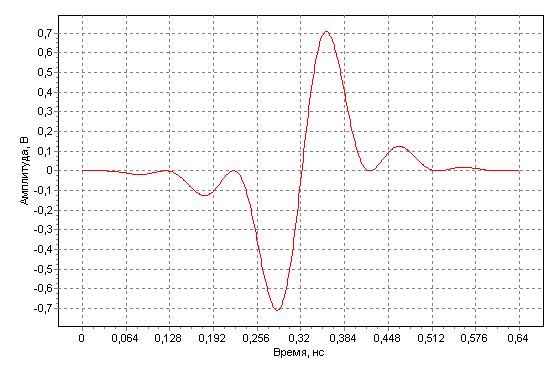
\includegraphics[width=0.7\textwidth]{graphics/tem-horn-vswr-signal}
\caption{СШП импульс, возбуждающий антенну.}
\label{fig:HornAntennaExitationSignal}
\end{figure}

% --- Рисунок
\begin{figure}[p]
\centering
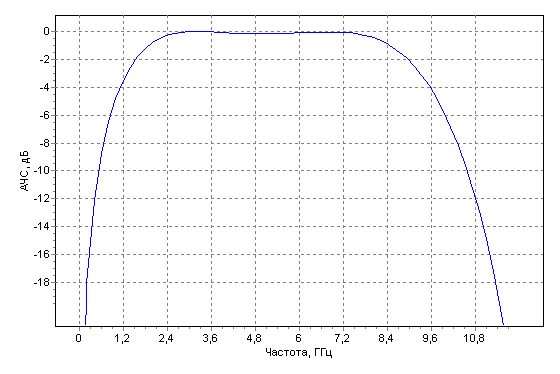
\includegraphics[width=0.7\textwidth]{graphics/tem-horn-vswr-signal-spectrum}
\caption{Амплитудно-частотный спектр импульса на
         рис.~\eqref{fig:HornAntennaExitationSignal}.}
\label{fig:HornAntennaExitationSignalSpectrum}
\end{figure}


% --- Рисунок
\begin{figure}[p]
\centering
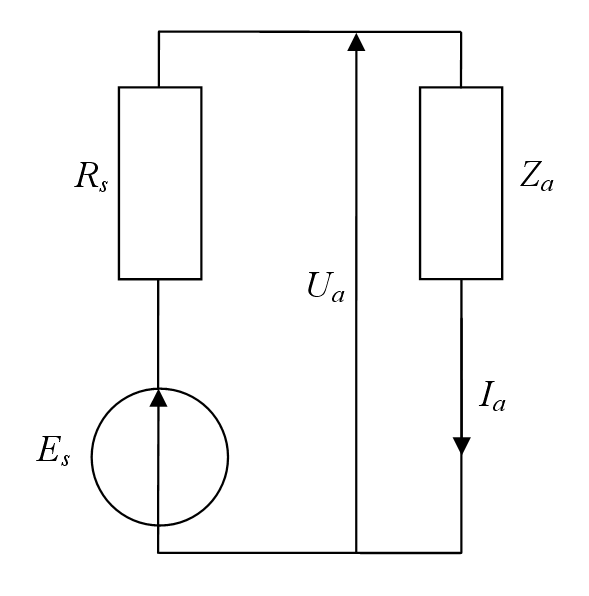
\includegraphics[width=0.3\textwidth]{graphics/horn-equivalent-scheme}
\caption{Эквивалентная схема для расчета волнового сопротивления
         антенны ($R_s=\valu{50}{Ом}$).}
\label{fig:HornAntennaEquivalentScheme}
\end{figure}

% --- Рисунок
\begin{figure}[p]
\centering
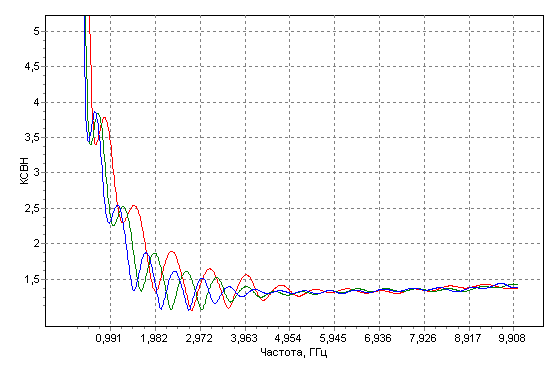
\includegraphics[width=\textwidth]{graphics/horn-vswr}
\caption{Зависимости КСВН от частоты для трех антенн различной длины:
         $R=\valu{150}{мм}$ (красный),
         $R=\valu{180}{мм}$ (зеленый)
       и~$R=\valu{200}{мм}$ (синий)}
\label{fig:HornAntennaVSWR}
\end{figure}

% --- Таблица
\begin{table}[tb]
\caption{
    Параметры пространственной сетки и PML, использованные при моделировании
    TEM-рупорных антенн.}
\label{tab:GridParameters}

\newcolumntype{C}{>{\centering\arraybackslash}X}
\begin{tabularx}{\textwidth}{|C|C|C|C|C|}
\hline
    Координата & Шаг, мм & R, \% & Слоев $N$ & Параметр~$g$ \\
\hline
    $x$ & \val{0.50} & \val{0.01} & \val{8} & \val{2.8} \\
    $y$ & \val{0.77} & \val{0.01} & \val{8} & \val{2.6} \\
    $z$ & \val{0.20} & \val{0.01} & \val{8} & \val{31} \\
\hline
\end{tabularx}
\end{table}

% --- Таблица
\begin{table}[tb]
\caption{Расчетные значения граничной частоты для ТЕМ-рупоров.}
\label{tab:ThresholdFrequency}

\newcolumntype{C}{>{\centering\arraybackslash}X}
\begin{tabularx}{\textwidth}{|l|C|C|C|}
    \hline
    \multirow{2}{*}{Уровень КСВН} &
    \multicolumn{3}{c|}{Граничная частота для разных ТЕМ-рупоров, ГГц} \\
    \cline{2-4}
    & $R=\valu{150}{мм}$ & $R=\valu{180}{мм}$ & $R=\valu{200}{мм}$ \\
    \hline
    4 (60\% отражения) & 0,55 & 0,48 & 0,43 \\
    3 (50\% отражения) & 1,05 & 0,88 & 0,80 \\
    2 (33\% отражения) & 1,71 & 1,47 & 1.32 \\
    \hline
\end{tabularx}
\end{table}


    \chapter{Энергетические диаграммы направленности TEM-рупорных антенн}
    

\section{Нахождение поля в дальней зоне}

Описанные в разделе~\ref{section:CoreMethod} работы методы численного решения
уравнений Максвелла вместе с описанными в разделе~\ref{section:GridReduction}
методами решения задач на открытых обласях дают возможность вычисления
электромагнитного поля внутри некоторой ограниченной области пространства.
Однако на размер этой области накладываются ограничения, вызванные конечной
вычислительной мощностью современных ЭВМ, а~именно тремя основными факторами:
\begin{itemize}
\item ограниченной скоростью выполнения арифметических операций;
\item ограниченным объемом оперативной памяти;
\item ограниченной скоростью обмена данными между процессором
      и оперативной памятью.
\end{itemize}
Однако, существует ряд задач, в~которых необходим расчет электромагнитных полей
на~больших расстояниях (в дальней зоне) от~некоторого объекта, излучающего или
рассевающего электромагнитное поле. В~число этих задач входит, например,
получение диаграмм направленности антенн.

Для решения подобных задач существует эффективный способ вычисления полей
в~дальней зоне с~использованием результатов вычисления поля в ближней зоне,
выполненного методом FDTD. Этот способ заключается в~использовании
поверхностного интеграла Кирхгоффа.

Интеграл Кирхгофа связывает поле внутри ограниченного объема с~полем и~его
производными на~поверхности, ограничивающей объем. Эта формула была выведена
в~середине XIX~века немецким физиком Гюставом~Кирхгофом, и~во~временной области
имеет следующий вид:
\begin{equation}
    \label{eq:KirchhoffIntegral}
    \Psi(\vect{p},t) = \frac{1}{4\pi} \oint_\Gamma
    \left[
        \frac{1}{R}\nabla'\Psi(\vect{p'},t') -
        \frac{\vect{R}}{R^3}\Psi(\vect{p'},t') -
        \frac{\vect{R}}{cR^2}\frac{\partial}{\partial t'}\Psi(\vect{p'},t')
    \right]_\text{ret} \!\!\!\!\!\vect{n} dA'.
\end{equation}

\noindent
В этом выражении используются обозначения:
\begin{where}
\item $\Psi$ --- любая из шести компонент поля;
\item $\Gamma$ --- поверхность, ограничивающая объем в ближней зоне;
\item $dA'$ --- площадь элемента поверхности;
\item $\vect{n}$ --- единичный вектор нормали к~поверхности;
\item $\vect{p}$ --- точка наблюдения в дальней зоне;
\item $\vect{p'}$ --- точка на~поверхности;
\item $R$ --- расстояние между ними, $\vect{R} = \vect{p}-\vect{p'}$;
\item $c$ --- скорость света в вакууме.
\end{where}

\noindent
В~формуле~\eqref{eq:KirchhoffIntegral} индекс «ret» обозначает тот факт, что
интегрирование осуществляется с~учетом запаздывающего времени~$t'=t-R/c$. Также
отметим, что единичный вектор нормали~$\vect{n}$ всегда направлен внутрь
рассматриваемого замкнутого объема.

Формула~\eqref{eq:KirchhoffIntegral} выражает принцип Гюйгенса, согласно
которому каждая точка на волновом фронте служит фиктивным источником
воображаемой сферической волны. Каждый участок поверхности~$dA'$ излучает волну,
которая приходит в~точку наблюдения с~задержкой~$R/c$. При этом на каждом шаге
FDTD по времени на поверхности интегрирования возникает совокупность фиктивных
источников, поле от которых придет в~точку наблюдения с~разным запаздыванием,
поскольку расстояние~$R$ для всех точек различно. Это означает, что на одном
временном шаге находятся вклад элемента площади~$dA'$ в~разные временные участки
выходного сигнала в~точке наблюдения.

Шаг по времени при вычислении интеграла Кирхгофа тесно связан с~шагом по времени
FDTD и равен ему. Выходная последовательность в~точке наблюдения имеет такой же
шаг по времени. Однако величина~$R/c$ может не быть кратной шагу по времени,
поэтому получаемое время задержки округляется до ближайшего значения, кратного
шагу FDTD. Возникающая при этом ошибка незначительна, т.к. временной шаг
в~классическом FDTD мал по сравнению с~периодом колебаний вычисляемого сигнала.

Выражение~\eqref{eq:KirchhoffIntegral} в~такой форме неудобно для совместного
применения с~методом FDTD. Вывод формул, используемых на~практике, в~данной
работе не приводится и может быть найден, например, в~\cite{bib:Zelenin2006}.
Отметим также, что для получения лучших результатов поверхность интегрирования
следует располагать не в~непосредственной близости от исследуемого объекта, а~на
некотором отдалении от него (порядка 10~шагов дискретизации по~пространству).

	
\section[Энергетические диаграммы направленности]
        {Энергетические диаграммы направленности и~импульсные характеристики антенн}
\label{div:DirectionalPatternsTheory}

Известно, что описание излучения импульсов субнаносекундной длительности имеет
особенности, связанные с~частотным составом излучаемого сигнала и~соотношением
протяженностей антенны и~излучаемого импульса. Так, полоса частот в~несколько
гигагерц делает неудобными для анализа характеристик излучения антенны
традиционные диаграммы направленности, применяемые для узкополосных
сигналов~\cite{bib:Immoreev2002}. Одна и~та же антенна на~частотах, отличающихся
в~несколько раз, может иметь совершенно разные характеристики излучения.

Кроме того, пространственная длительность импульса может не~превышать
протяженности излучающей части антенны. В~подобных случаях форма сигнала может
существенно зависеть от~угла наблюдения. При этом форма сигнала в~заданной точке
пространства не~может быть описана только усилением в~заданном направлении.
Таким образом, для того чтобы описать процесс излучения импульса антенной,
необходимо несколько характеристик~\cite{bib:Immoreev2002,bib:Astanin1989}:
\begin{itemize}
\item
энергетические диаграммы направленности, которые характеризуют усредненное
пространственное распределение энергии за~все время существования излучаемого
сигнала;
\item
набор импульсных характеристик антенны, которые позволяют оценить форму импульса
в~заданной точке пространства по~входному сигналу произвольной формы.
\end{itemize}

Для расчета энергетических диаграмм направленности использовались данные
моделирования поля в~дальней зоне. Так как энергии электрической и~магнитной
составляющих поля равны, усредненная энергия ТЕМ-волны за~время существования
импульса в~заданной точке пространства может быть рассчитана по~электрической
составляющей с~помощью следующего соотношения:
\begin{equation}
    \label{eq:AverageWaveEnergy}
    W(r,\theta,\phi) = C\hanglimitsoperator{\int}{R/c+T}{R/c}
    \left| E_\theta(r,\theta,\phi) \right|^2 dt,
\end{equation}
где $c$ --- скорость света в~свободном пространстве, $T$ --- длительность
сигнала в~заданной точке дальней зоны. Далее проводилась нормировка на~максимальное значение
(поэтому в~расчетах было принято, что~$C=1$). Как видно
из~\eqref{eq:AverageWaveEnergy}, расчет энергетических диаграмм направленности
связан с~оценкой электрической составляющей поля в~заданной точке пространства.
При этом вызывает интерес оценка характеристик антенны при излучении сигналов
различной формы. В~этом случае пересчет поля в~дальней зоне может быть
осуществлен без~полного электродинамического моделирования, которое для
крупногабаритных антенн может занять значительное время. Достаточно точно
оценить отклик в~любой точке пространства можно, зная импульсную характеристику
системы <<антенна–пространство>> для данных координат.

Так как антенна и~окружающая среда линейны, связь между сигналом, возбуждающим
антенну, и~полем в~заданной точке пространства можно записать в~виде:
\begin{equation}
    \label{eq:TangentialElectricField}
	E_\theta(r,\theta,\phi,t) = h(r,\theta,\phi,t) * s(t),
\end{equation}
где $h(r,\theta,\phi,t)$ --- импульсная характеристика, $s(t)$ --- сигнал на~входе
антенны, а~звездочкой обозначен оператор свертки по времени.

Если импульсная характеристика в~заданной точке пространства известна, то
с~помощью соотношения~\eqref{eq:TangentialElectricField}, можно рассчитать
электрическую составляющую поля в~этой точке. Если же ее требуется найти, то
соотношение~\eqref{eq:TangentialElectricField} следует рассматривать как
линейное уравнение относительно $h(r,\theta,\phi,t)$. Проведя моделирование
с~тестовым сигналом~$s(t)$, можно рассчитать электрическую составляющую поля
в~заданной точке, и, решив~\eqref{eq:TangentialElectricField},
найти~$h(r,\theta,\phi,t)$.

Имея набор импульсных характеристик в~заданных точках пространства, можно
рассчитать энергетические диаграммы направленности для различных сигналов,
не~прибегая к~полному электродинамическому моделированию антенны.

	%
%
%
\section{Расчет диаграмм направленности TEM-рупорных антенн}

Из-за большой ширины спектра сигналов, используемых в сверхширокополосных
радиосистемах на СКИ, описание антенны при помощи диаграмм направленности,
используемых обычно в случае узкополосных сигналов, не имеет смысла, так как вид
диаграммы направленности антенны может кардинальным образом образом отличаться
на разных частотах, входящих в спектр СКИ. Поэтому  выглядит целесообразным
использование в этом случае энергетических диаграмм направленности, выражающих
полную энергию, пришедшуюся на то или иное направление за всё время излучения.
Среди пригодных для излучения и приема СКИ сигналов антенн можно выделить
ТЕМ-рупоры с переменным волновым сопротивлением, изменяющимся, как правило,
от~\valu{50}{Ом} в~точке запитки до~$120\pi\,Ом$
у~раскрыва~\cite{bib:Aizenberg1985}. По сути, такая антенна представляет собой
переход с плавно изменяющимся волновым сопротивлением (\emph{плавный переход}).
Однако, форма раскрыва такой рупорной антенны может быть различной. Далее
в~работе рассматриваются два типа антенн: с линейным и экспоненциальным профилем
раскрыва, и исследовалось влияние формы антенны на направленность.

Несмотря на то, что геометрия подобных антенн сложна для аналитических
вычислений, она поддается анализу с помощью численных методов. С помощью метода
FDTD было проведен расчет синтезированных рупоров во временной области, были
построены и проанализированы энергетические диаграммы направленности для
различных сигналов. При этом полное электродинамическое моделирование
выполнялось лишь для одного сигнала, затем по полученному отклику антенны
находились характеристические функции, позволяющие в дальнейшем находить отклик
антенны на сигнал произвольной формы.


\subsection{Вывод уравнений профиля антенны}

Получим выражения, описывающие профиль рупорных антенн с~экспоненциальным
и~линейным раскрывами. Прежде всего введем систему прямоугольных координат.
Пусть антенна расположена симметрично относительно оси~$O_x$ и~главное
направление излучения антенны совпадает с~направлением этой оси, входу антенны
соответствует координата $x=0$. Лепестки антенны расположены симметрично
друг другу относительно плоскости Oxy. Тогда можем записать выражения для
расстояния между лепестками:
\begin{align}
	\label{eq:LinearProfile}
    H(x) &= H_0 + (H_R-H_0)\frac{x}{R}, && \text{(линейный раскрыв)} \\
    \label{eq:ExponentialProfile}
    H(x) &= H_0 \exp
    \left[
        \left(\frac{x}{R}\right)^\alpha\ln\frac{H_R}{H_0}
    \right] && \text{(экспоненциальный раскрыв~\cite{bib:Karshenas2009})}
\end{align}

\noindent
В этих формулах:
\begin{where}
\item $H_0$ --- расстояние между лепестками в~начале раскрыва;
\item $H_R$ --- расстояние между лепестками в~конце раскрыва;
\item $R$ --- длина раскрыва антенны вдоль координаты~$x$.
\end{where}

\noindent
Будем считать антенну длинной линией с~распределенными параметрами, фактически
--- полосковой линией с~переменными шириной и~расстоянием между проводниками.
В~\cite{bib:Aizenberg1985} показано, что уровень отражения входного сигнала
в~длинной линии получается наименьшим, если ее волновое сопротивление изменяется
в~пространстве по~экспоненциальному закону от~входного сопротивления антенны
до~сопротивления нагрузки на~выходе антенны. Итак, волновое сопротивление антенн
(с~обоими рассматриваемыми типами раскрыва) имеет вид:
\begin{equation}
    \label{eq:HornWaveResistance}
    Z(x) = Z_0 \exp
    \left[
        \left(\frac{Z_R}{Z_0}\right)
        \frac{x}{R}
    \right],
\end{equation}
где $Z_0$ --- входное сопротивление антенны, $Z_R$ --- сопротивление нагрузки,
на~которую выполняется согласование.

Теперь воспользуемся известным соотношением для волнового сопротивления
полосковой линии:
\begin{equation}
    \label{eq:MicrostripWaveResistance}
    Z = \frac{H\zeta_0}{B},
\end{equation}
%
\begin{where}
\item $H$ --- расстояние между проводниками линии;
\item $B$ --- ширина проводников;
\item $\zeta_0=120\pi$ --- т.~н. волновое сопротивление вакуума.
\end{where}

\noindent
В~нашей задаче $H$ и~$B$ не~являются постоянными, кроме того, нас интересует
значение ширины лепестка антенны, поэтому выразим его из
формулы~\eqref{eq:MicrostripWaveResistance}:
\begin{equation}
    \label{eq:ProfileWidthFromWaveResistance}
    B(x) = \frac{H(x)\zeta_0}{Z(x)}.
\end{equation}

Подставляя~\eqref{eq:LinearProfile} и~\eqref{eq:ExponentialProfile}
в~\eqref{eq:ProfileWidthFromWaveResistance}, получим после несложных
преобразований окончательные выражения для ширины лепестков антенн:
\begin{align}
    % --
    \label{eq:LinearProfileWidth}
    B(x) &= \frac{\zeta_0}{Z_0}
    \left[ H_0 + (H_R-H_0)\frac{x}{R} \right]
    \exp\left[
        -\frac{x}{R}\ln\frac{Z_R}{Z_0}
    \right] & \text{(линейный)} \\
    % --
    \label{eq:ExponentialProfileWidth}
    B(x) &= \frac{H_0\zeta_0}{Z_0}
    \exp\left[
        \left(\frac{x}{R}\right)^\alpha \ln\frac{H_R}{H_0} -
        \frac{x}{R} \ln\frac{Z_R}{Z_0}
    \right] & \text{(экспоненциальный)}
\end{align}

Это и~есть искомые профили антенн. Графики этих зависимостей при различных
значениях параметра~$Z_R$ изображены на~рис.~\ref{fig:ProfileWidths}
в~разделе~\ref{div:DirectionalPatternExperimentDescription}.


\subsection{Постановка задачи}

Была поставлена задача провести исследование характеристик TEM-рупорных антенн
с~линейным и~экспоненциальным раскрывами. Требуемые выходные сопротивления
антенн:
    \val{150}, \val{200}, \val{250},
    \val{300}, \val{350}, \val{377},
    \val{450}, \valu{500}{Ом}.
(Величина \valu{377}{Ом}, приблизительно равная так называемому волновому
сопротивлению вакуума, взята вместо наиболее близкого к~нему
значению~\valu{400}{Ом} из арифметической прогрессии.) Для каждого значения
выходного сопротивления из этого списка требовалось синтезировать пару рупорных
антенн: с~линейным и~экспоненциальным раскрывами. При этом для всех антенн
неизменными оставались следующие параметры:
\begin{itemize}
\item длина антенны (вдоль оси~$x$):                 $R=\valu{125}{мм}$;
\item расстояние между лепестками в~начальной точке: $H_0=\valu{2}{мм}$;
\item расстояние между лепестками в~конечной точке:  $H_R=\valu{75}{мм}$;
\item параметр~$\alpha$ из
      формулы~\eqref{eq:ExponentialProfile}:         $\alpha=1$;
\item входное сопротивление антенны:                 $Z_0=\valu{50}{Ом}$.
\end{itemize}

\noindent
Требовалось найти отклик антенн и~энергетические диаграммы направленности для
гауссовских униполярных импульсов длительностью~\valu{100}{пс}, \valu{400}{пс}
и~\valu{1000}{пс}.


\subsection{Описание численного эксперимента}
\label{div:DirectionalPatternExperimentDescription}

Для численного эксперимента использовался метод конечных разностей во~временной
области (FDTD) и~его расширения, в~частности, использованы граничные условия
типа идеально согласованного слоя (PML) и~преобразование ближнего поля в~дальнее
(NF-to-FF) при помощи интеграла Кирхгофа. Для этого использовалась программа
\emph{Fdtd3d}, написанная аспирантом кафедры электроники физического факультета
ВГУ Мещеряковым И.\,И. Прежде всего были найдены профили всех антенн. Так,
расстояние между лепестками в~зависимости от~продольной координаты задается
с~помощью формул~\eqref{eq:LinearProfile} и~\eqref{eq:ExponentialProfile}.
Ширина самих лепестков находилась из
соотношения~\eqref{eq:MicrostripWaveResistance} и~задается выведенными там же
формулами~\eqref{eq:LinearProfileWidth} и~\eqref{eq:ExponentialProfileWidth}.
Графики функций~$B(x)$ при различных значениях параметра~$Z_R$ приведены
на~рис.~\ref{fig:ProfileWidths}. Геометрия исследуемых антенн аппроксимировалась
в~счетной области прямоугольными ячейками. Величины шагов дискретизации
по~пространству были выбраны следующими:
\begin{itemize}
\item по оси~$x$: $\Delta{x}=\valu{1.00}{мм}$;
\item по оси~$y$: $\Delta{y}=\valu{1.54}{мм}$;
\item по оси~$z$: $\Delta{z}=\valu{0.50}{мм}$.
\end{itemize}
Шаг дискретизации по~времени рассчитывался автоматически из~условия
Куранта~\eqref{eq:CourantCondition}.

Материал антенны --- медь ($\sigma_E=\valu{5.8E7}{Ом^{-1}}$), а окружающая среда
--- вакуум. В начале раскрыва антенны был установлен ряд точечных резистивных
источников напряжения, на~которые подавался входной сигнал. Для возбуждения
антенны использовался униполярный гауссовский сигнал
длительностью~\valu{100}{пс}. График этого сигнала приведен на
рис.~\ref{fig:DirectionalPatternsSignals}. Для построения диаграммы
направленности вне счетного объема были установлены пробники типа~NF-FF,
распределенные в~плоскостях $O_{xy}$ и~$O_{xz}$ по двум окружностям
радиусом~\valu{30}{м} с~шагом 5~градусов. При этом, в~силу симметрии задачи
и~так как поле позади антенны нас не~интересует, пробники распределялись только
по~четверти длины окружностей. Сама же антенна окружалась прямоугольной
поверхностью, отстоящей от~антенны на 10~шагов дискретизации по~пространству.
По~этой поверхности производилось интегрирование для преобразования ближних
полей в~дальнее. Границы PML отстояли от~поверхности интегрирования еще на
10~шагов дискретизации. Схема эксперимента приведена
на~рис.~\ref{fig:DirectionalPatternExperiment}.


\subsection{Полученные результаты}

После завершения моделирования были получены значения электромагнитных полей
на~пробниках в~каждой временной итерации. Эти значения были были использованы
для построения диаграмм по~методике, описанной
    в~разделе~\ref{div:DirectionalPatternsTheory}
    и~\cite{bib:MescheryakovUnpublishedReport},
а~также для расчета отклика антенны и~её диаграмм направленности при других
входных сигналах при помощи импульсных характеристик. Для упрощения анализа
проведем сравнение только двух антенн: с~выходным волновым сопротивлением
\valu{377}{Ом} и~разными типами раскрыва. В~дальнейшем все графики относятся
именно к~этим антеннам.

Графики тока и~напряжения, полученные на~выходе антенн при моделировании
(на вход антенны подавался сигнал длительностью \valu{100}{нс}) приведены
    на~рис.~\ref{fig:ReplyVoltages377}
    и~\ref{fig:ReplyCurrents377}.
Полученные диаграммы направленности приведены:
\begin{itemize}
\item для сигнала длительностью~\valu{100}{пс} (исходного) ---
      на~рис.~\ref{fig:DirectionalPattern100ps};
\item для сигнала длительностью~\valu{400}{пс} ---
      на~рис.~\ref{fig:DirectionalPattern400ps};
\item для сигнала длительностью~\valu{1000}{пс} ---
      на~рис.~\ref{fig:DirectionalPattern1000ps}.
\end{itemize}


\subsection{Анализ полученных результатов}

Обратимся к~диаграммам направленности. Можно видеть, что антенна
с~экспоненциальным профилем раскрыва обладает значительно более узкой диаграммой
направленности в~вертикальной плоскости и~в~то же время более широкой диаграммой
в~горизонтальной плоскости.

\paragraph{Излучение сигнала длительностью~100~пс.\\}
Пространственная длительность данного сигнала меньше длины антенны. В~этом
случае антенна с~экспоненциальным раскрывом обладает значительно лучшей
направленностью как по углу~$\phi$, так и~по углу~$\theta$.

\paragraph{Излучение сигнала длительностью~400~пс.\\}
Пространственная длительность данного сигнала примерно соответствует длине
антенны. В~этом случае направленность антенны с~экспоненциальным профилем
по~углу~$\theta$ по-прежнему значительно лучше, чем антенны с~линейным
раскрывом. В~то же время направленность по углу~$\phi$ экспоненциальной антенны
несколько хуже, чем линейной.

\paragraph{Излучение сигнала длительностью~1000~пс.\\}
Пространственная длительность данного сигнала значительно больше длины антенны.
Направленность антенны с~экспоненциальным профилем как по~$\phi$, так
и~по~$\theta$ значительно ухудшилась по~сравнению с~антенной с~линейным
профилем.

Из сказанного заключим, что применение антенн с~экспоненциальным раскрывом
вместо антенн с~линейным раскрывом более собразно при использовании сигналов
с~пространственной длительностью, меньшей длины антенны.

%% --
\begin{figure}
\label{fig:DirectionalPatternExperiment}
\centering
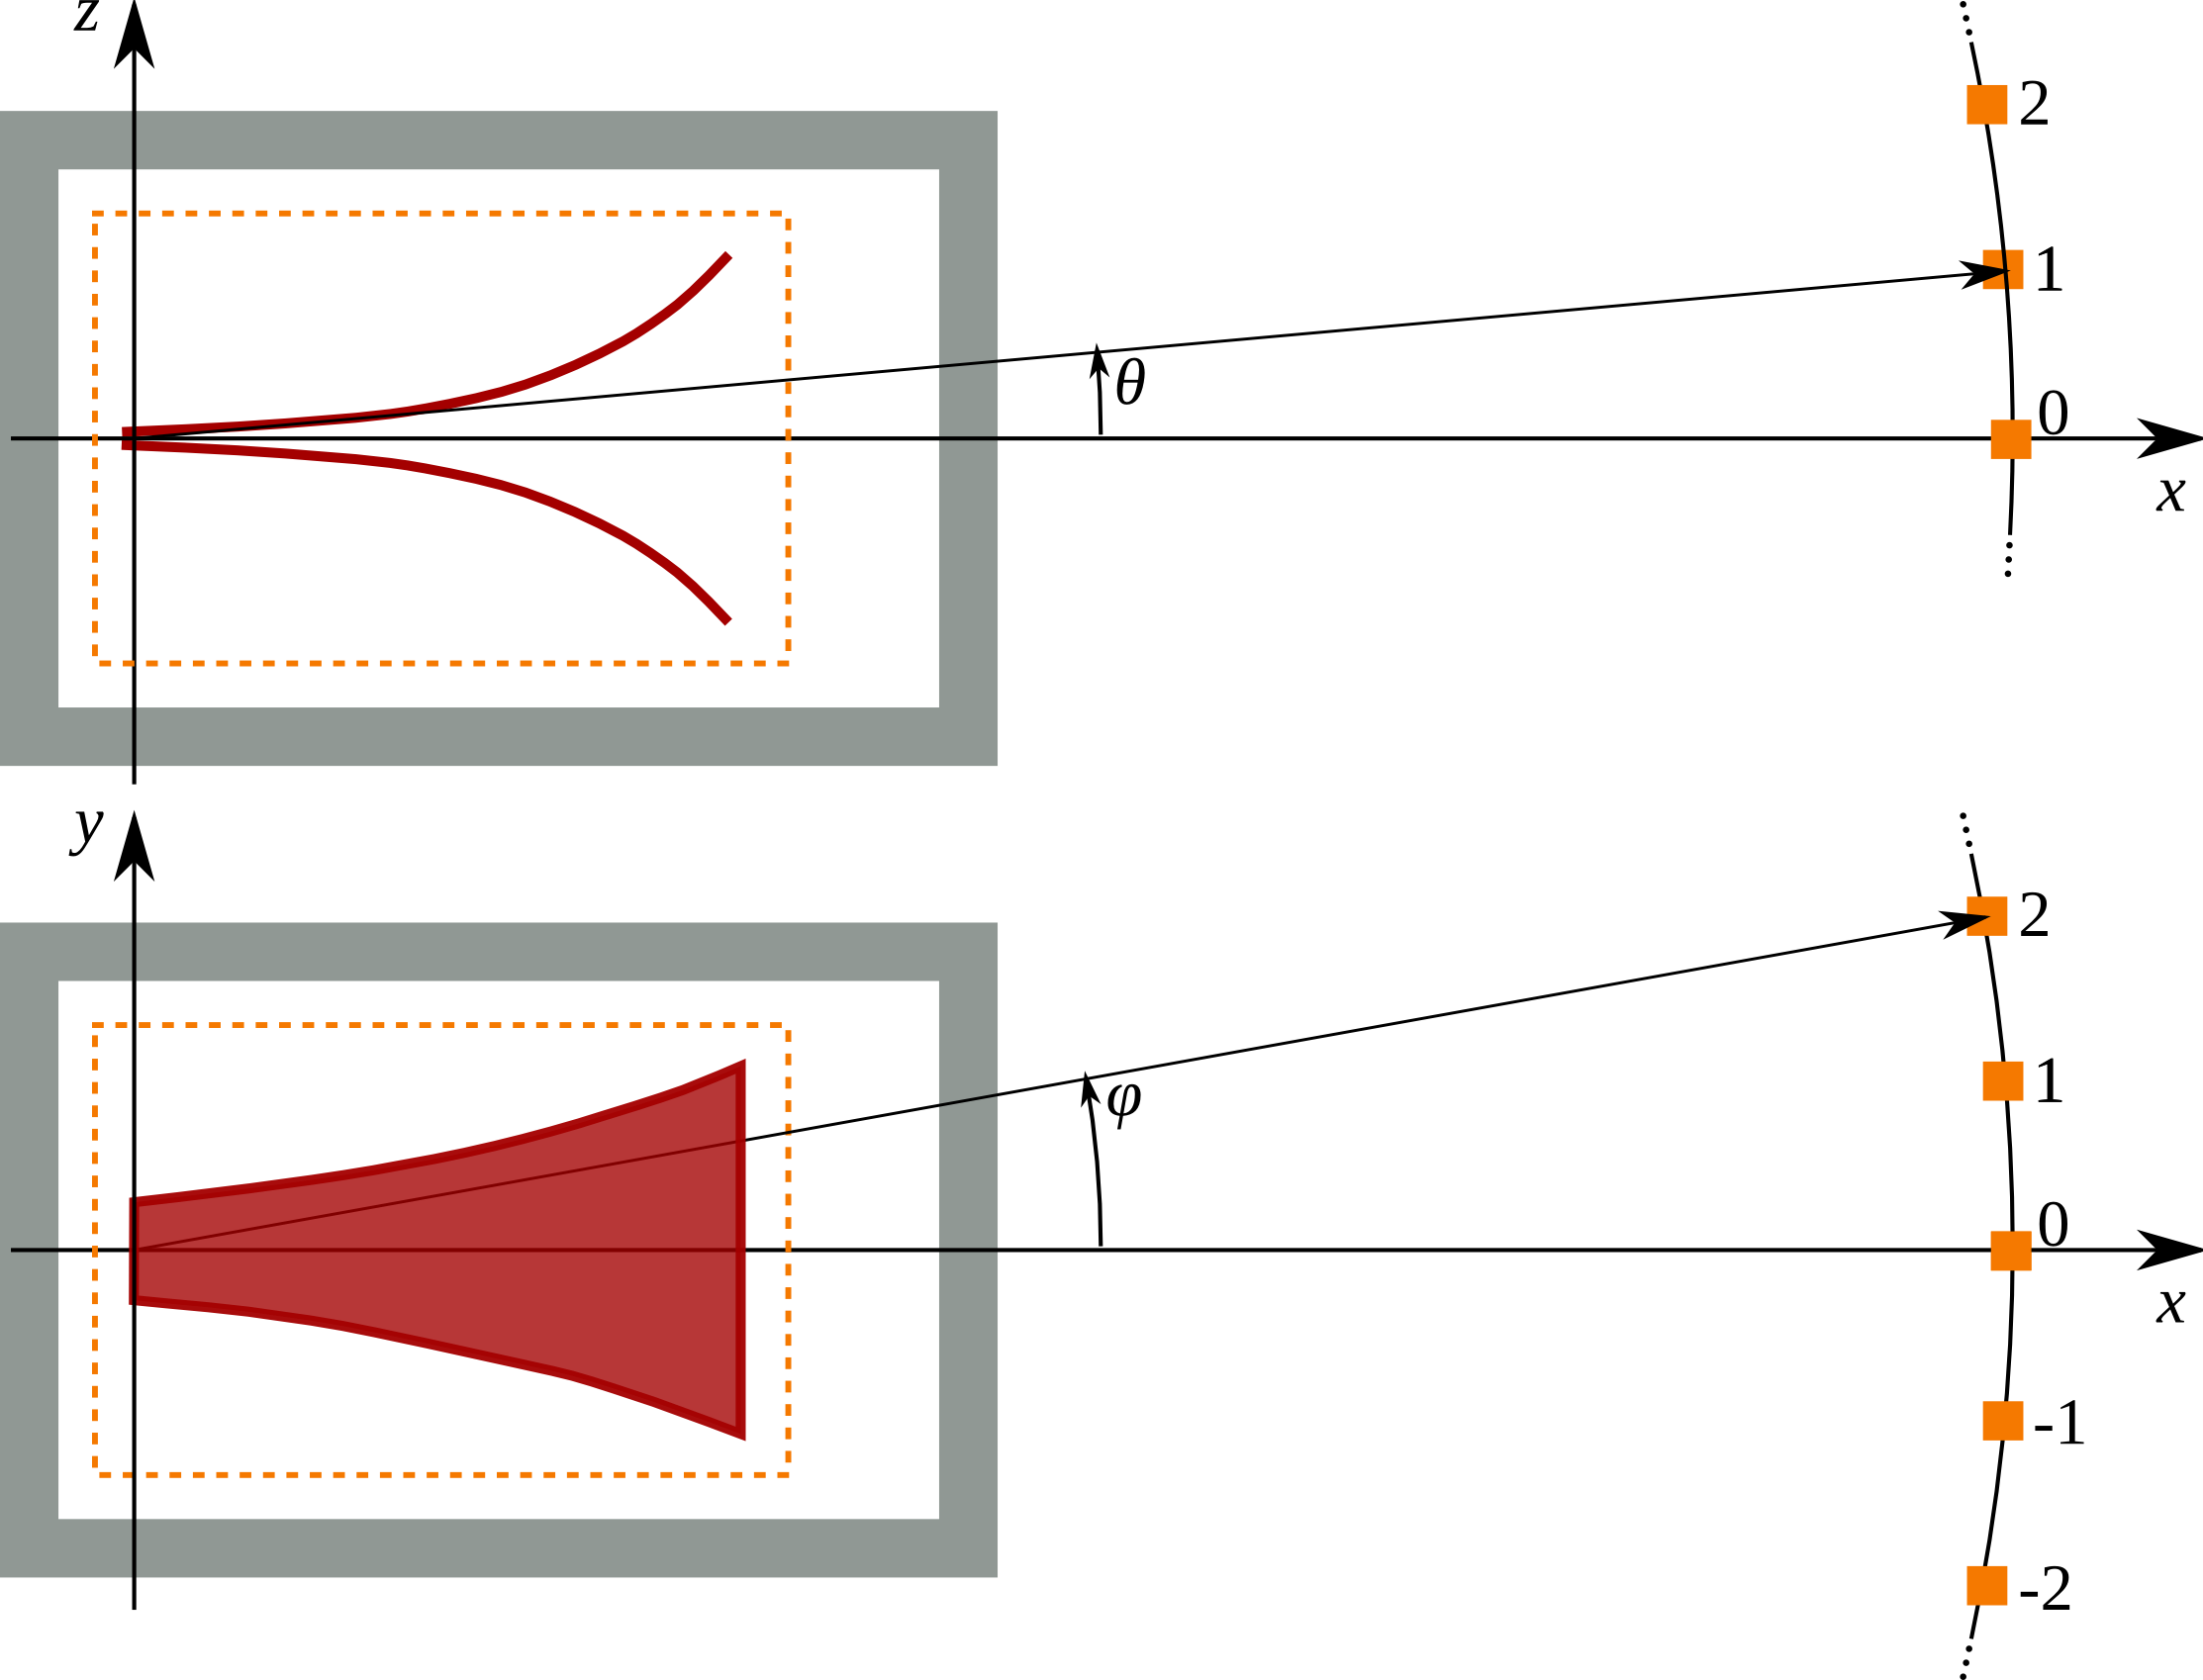
\includegraphics[width=0.7\textwidth]{graphics/directional-patterns-experiment-scheme}
\caption{
    Схема эксперимента, вид в~профиль (вверху), вид сверху (внизу).
    Прямоугольниками обозначены пробники для преобразования ближнего поля
    в~дальнее, пунктирная рамка обозначает поверхность интегрирования для
    интеграла Кирхгофа. Угловое расстояние между пробниками составляет
    5~градусов.}
\end{figure}

%% --
\begin{figure}
\label{fig:DirectionalPatternsSignals}
\centering
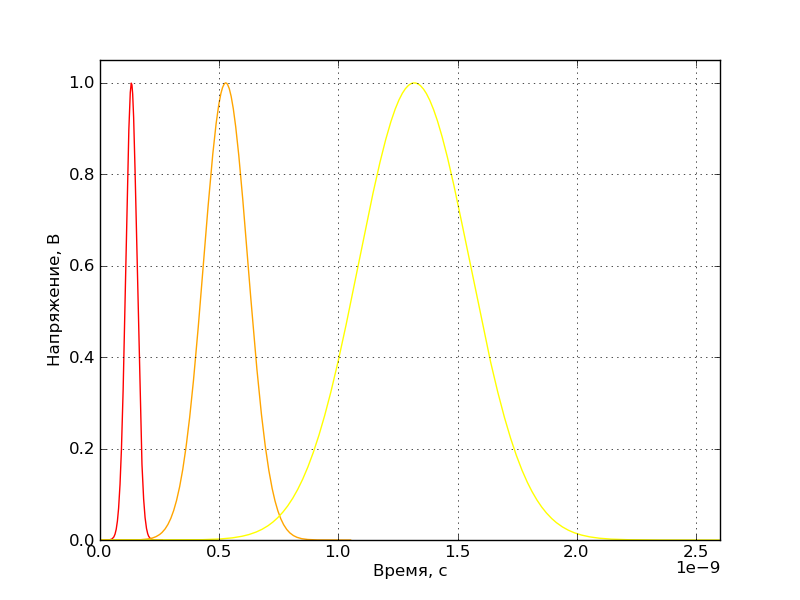
\includegraphics[width=0.7\textwidth]{graphics/directional-patterns-signals}
\caption{
    Входные сигналы антенны --- униполярные гауссовские импульсы различной
    длительности. Красная линия изображает сигнал длительностью~\valu{100}{пс},
    оранжевая --- длительностью~\valu{400}{пс},
    желтая --- длительностью~\valu{1000}{пс}.
    Длительность импульса определялась по~уровню 1/10.}
\end{figure}

%% --
\begin{figure}
\label{fig:ReplyVoltages377}
\centering
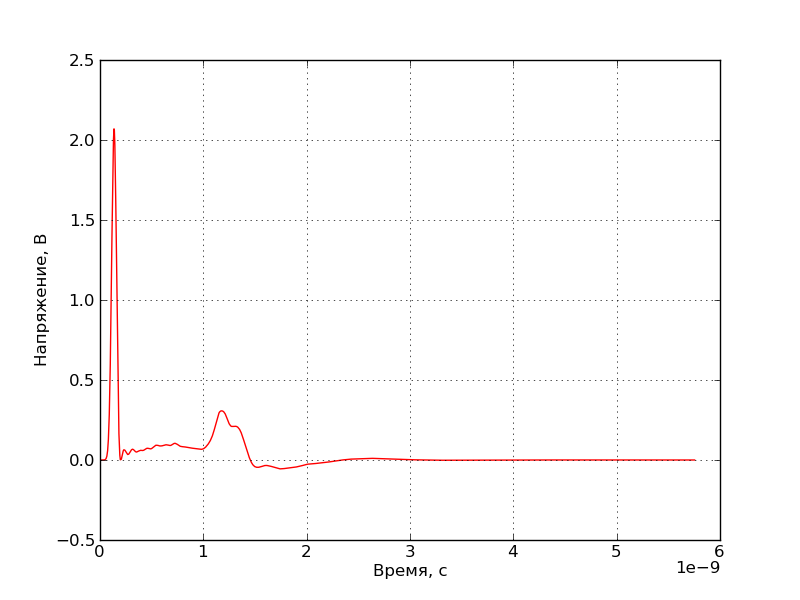
\includegraphics[width=0.7\textwidth]{graphics/directional-patterns-reply-linear-U}
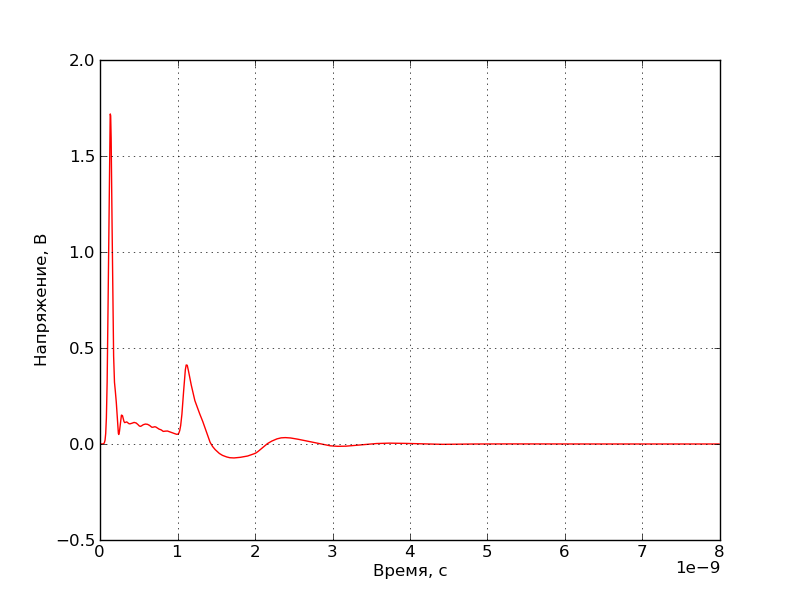
\includegraphics[width=0.7\textwidth]{graphics/directional-patterns-reply-exponential-U}
\caption{
    Напряжения на~выходе антенн с~линейным (вверху) и~экспоненциальным (внизу)
    профилями, синтезированными для выходного сопротивления~\valu{377}{Ом}.}
\end{figure}

%% --
\begin{figure}
\label{fig:ReplyCurrents377}
\centering
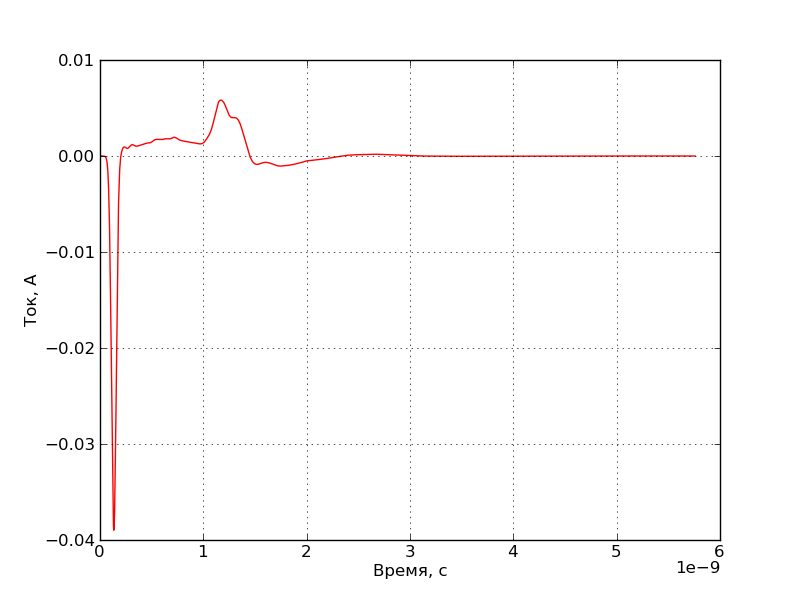
\includegraphics[width=0.7\textwidth]{graphics/directional-patterns-reply-linear-I}
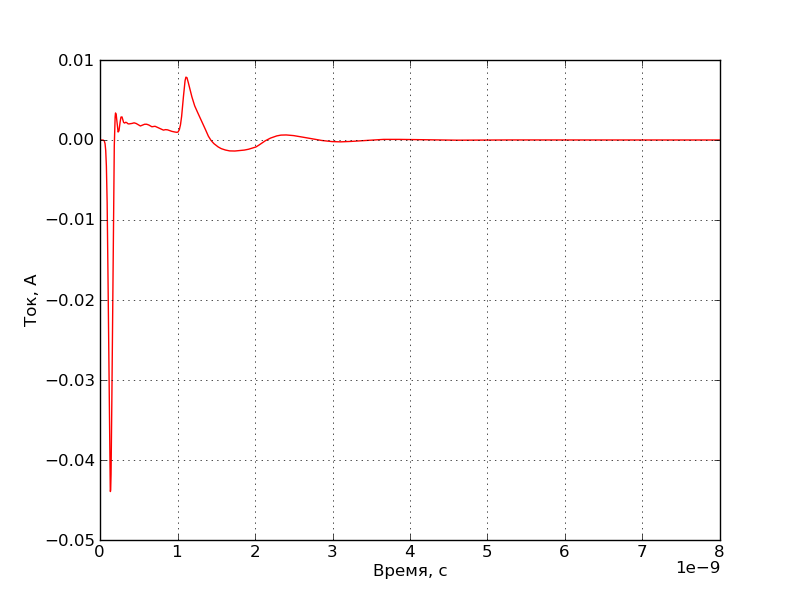
\includegraphics[width=0.7\textwidth]{graphics/directional-patterns-reply-exponential-I}
\caption{
    Токи на~выходе антенн с~линейным (вверху) и~экспоненциальным (внизу)
    профилями, синтезированными для выходного сопротивления~\valu{377}{Ом}.}
\end{figure}

%% --
\begin{figure}
\label{fig:ProfileWidths}
\centering
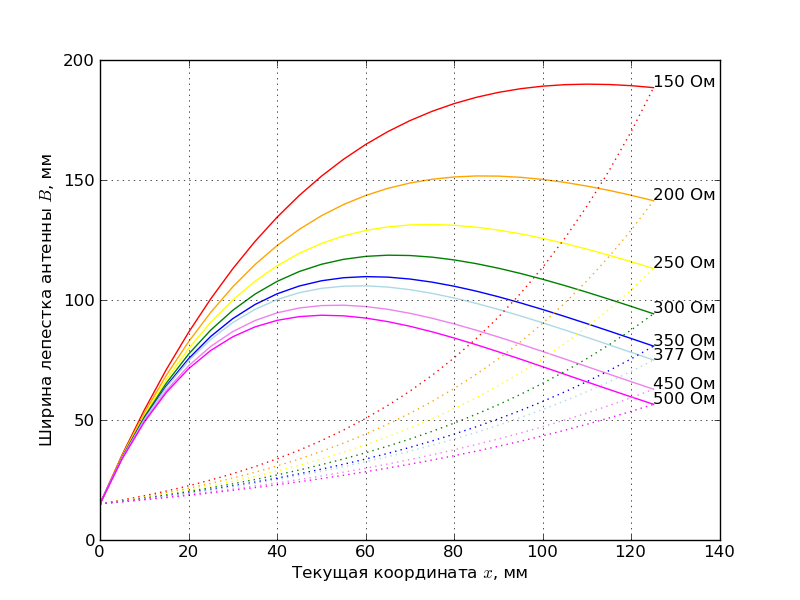
\includegraphics[width=0.7\textwidth]{graphics/directional-patterns-profile-widths}
\caption{
    Зависимость ширины лепестков исследуемых антенн от~значения продольной
    координаты при различных значениях параметра~$Z_R$. Сплошными линиями
    обозначены профили антенн с~линейным раскрывом, пунктирными --- профили
    антенны с~экспоненциальными раскрывами. Видно, что конечные точки профилей
    с~одинаковым волновым сопротивлением совпадают, как и~должно быть согласно
    теории. Подписи на~графике относятся к~паре антенн с~данной конечной точкой.}
\end{figure}

% ---
\begin{figure}
\label{fig:DirectionalPattern100ps}
\centering
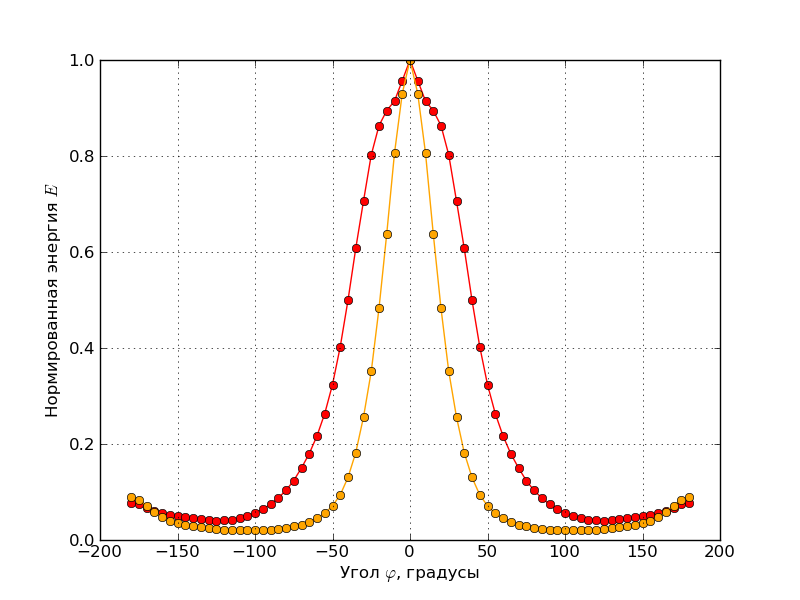
\includegraphics[width=0.7\textwidth]{graphics/directional-patterns-100ps-phi}
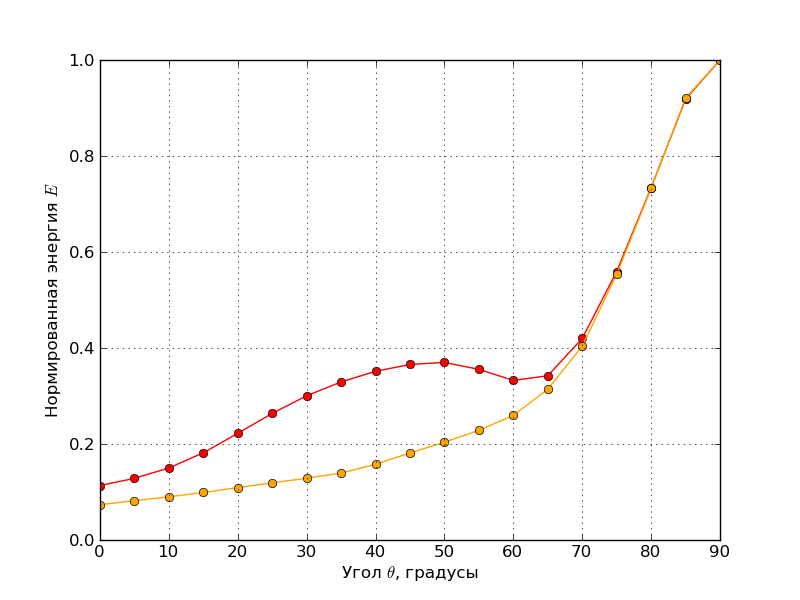
\includegraphics[width=0.7\textwidth]{graphics/directional-patterns-100ps-theta}

\caption{
    Сравнение энергетических диаграмм направленности в~горизонтальной (вверху)
    и~вертикальной плоскостях~(внизу) для двух антенн, синтезированных для
    выходного сопротивления~\valu{377}{Ом}, при возбуждении сигналом
    длительностью~\valu{100}{пс}. Красным цветом изображены диаграммы
    направленности антенны с~линейным раскрывом, оранжевым ---
    с~экспоненциальным.}
\end{figure}

% ---
\begin{figure}
\label{fig:DirectionalPattern400ps}
\centering
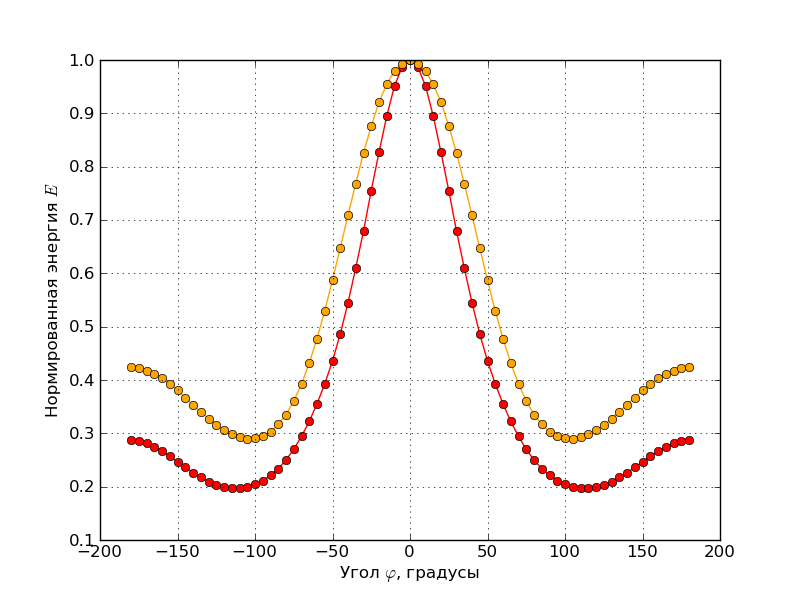
\includegraphics[width=0.7\textwidth]{graphics/directional-patterns-400ps-phi}
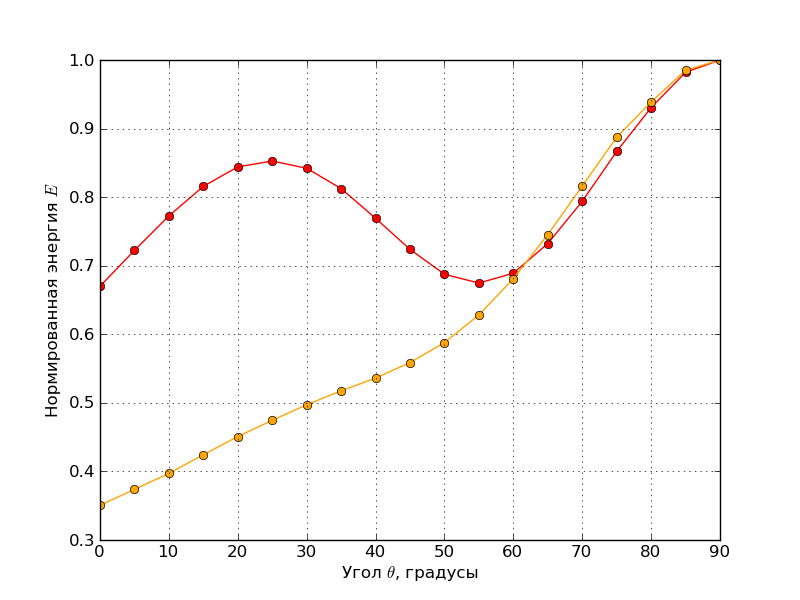
\includegraphics[width=0.7\textwidth]{graphics/directional-patterns-400ps-theta}

\caption{
    Сравнение энергетических диаграмм направленности в~горизонтальной (вверху)
    и~вертикальной плоскостях~(внизу) для двух антенн, синтезированных для
    выходного сопротивления~\valu{377}{Ом}, при возбуждении сигналом
    длительностью~\valu{400}{пс}. Красным цветом изображены диаграммы
    направленности антенны с~линейным раскрывом, оранжевым ---
    с~экспоненциальным.}
\end{figure}

% ---
\begin{figure}
\label{fig:DirectionalPattern1000ps}
\centering
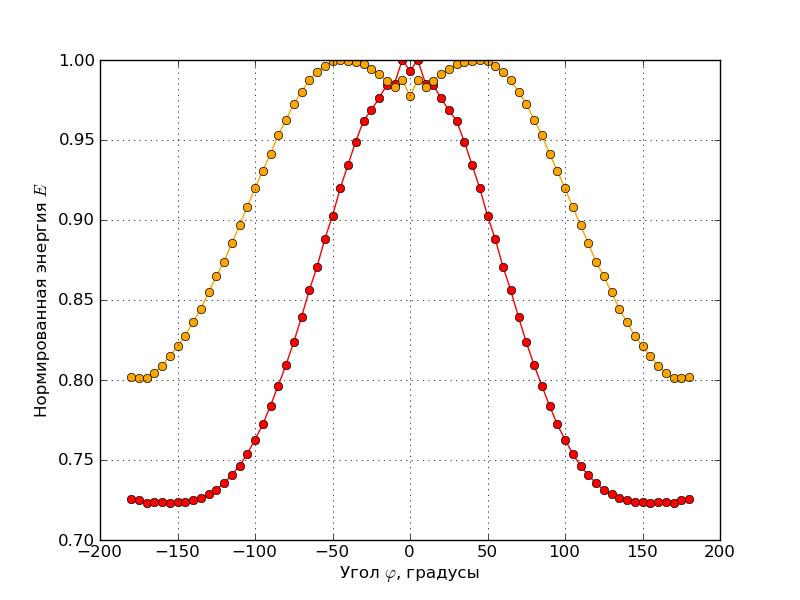
\includegraphics[width=0.7\textwidth]{graphics/directional-patterns-1000ps-phi}
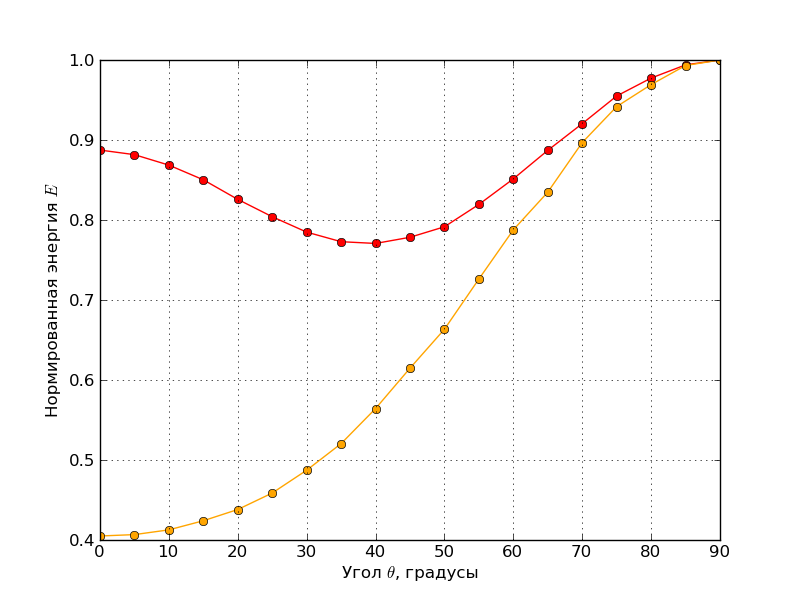
\includegraphics[width=0.7\textwidth]{graphics/directional-patterns-1000ps-theta}

\caption{
    Сравнение энергетических диаграмм направленности в~горизонтальной (вверху)
    и~вертикальной плоскостях~(внизу) для двух антенн, синтезированных для
    выходного сопротивления~\valu{377}{Ом}, при возбуждении сигналом
    длительностью~\valu{1000}{пс}. Красным цветом изображены диаграммы
    направленности антенны с~линейным раскрывом, оранжевым ---
    с~экспоненциальным.}
\end{figure}


	\chapter*{Заключение}
\addcontentsline{toc}{chapter}{Заключение}

В работе был рассмотрен метод конечных разностей во временной области, были
выведены его основные уравнения и указаны условия стабильности.
Кроме того, были указаны способы задания граничных условий и рассмотрены
системы идеально согласованных слоев. Хотя область применения метода довольно широка, особо
выигрышным представляется его использование при исследовании нестационарных
процессов --- например, электромагнитного поля антенн при возбуждении их
короткими импульсами.

Так, Было проведено моделирование трех ТЕМ-рупоров с~экспоненциальным профилем
изменения волнового
сопротивления, обладающих различной длиной. В~результате расчета были получены
зависимости КСВН от частоты в~диапазоне \val{0.1}--\valu{10}{ГГц}. При этом
нижняя граничная частота по уровню КСВН~4 уменьшается при увеличении длины
антенны. Полученная закономерность хорошо согласовывается с~выводами из теории
переходов с~плавным изменением волнового сопротивления. Следует отметить,
что увеличение длины ТЕМ-рупора на~\valu{3}{см}, что соответствует~20\% от
исходной длины~\valu{150}{мм}, позволило понизить нижнюю граничную частоту
приблизительно на~\valu{100}{МГц}, увеличение на~\valu{5}{см} (на~33\% от
исходной длины) --- на \valu{140}{МГц}, что представляет весьма важный
практический результат.

% -- Про диаграммы направленности
Также были промоделированы шестнадцать ТЕМ-рупоров с линейными
и экспоненциальными раскрывами. Полученные результаты моделирования
использовались для нахождения импульсных характеристик антенны и расчета ее
отклика на сигналы, форма которых отлична от используемой при фактическом
моделировании. В результате расчета были получены энергетические диаграммы
направленности излучения сигналов разной длительности для антенн с различными
профилями, выходными сопротивлениями (в целях краткости изложения, в работе
приведены диаграммы направленности только для двух антенн и трех сигналов).
Было установлено, что диаграммы направленности антенны с экспоненциальным
профилем раскрыва уже, чем у антенны с линейным раскрывом, в особенности при
излучении сигналов, пространственная длительность которых меньше размеров
антенны.


	
\nocite{bib:BobreshovKretov2011}
\nocite{bib:BobreshovKretov2012}

\begin{singlespacing}
\bibliography{bibliography/fdtd-theory,bibliography/hdf5}
\end{singlespacing}


    %\appendix
	%
\chapter{Ключевые фрагменты программного кода}

Ниже приведем некоторые фрагменты кода, отвечающие как за сериализацию в целом,
так и за работу непосредственно с форматом HDF~5 и использование
библиотеки \code{libhdf5}. В приложении представлен только код, отвечающий
за запись, т.~к. соответствующий код чтения во многом ему симметричен и может
быть опущен без ущерба для восприятия общей картины. Кроме того, опущены
реализации классов \code{HierarchyCrawler} и \code{SequentalWriter}, т.~к.
реализация первого достаточно объемна, а реализация второго --- практически
тривиальна.

\singlespacing

\subsubsection{HierarchyCrawler.h}
\lstinputlisting[language=c++]{appendix/HierarchyCrawler.h}

\subsubsection{SequentalWriter.h}
\lstinputlisting[language=c++]{appendix/SequentalWriter.h}

\subsubsection{HierarchyCrawlerImpl.h}
\lstinputlisting[language=c++]{appendix/HierarchyCrawlerImpl.h}

\subsubsection{SequentalWriterImpl.h}
\lstinputlisting[language=c++]{appendix/SequentalWriterImpl.h}

\subsubsection{HdfWriterImpl.h}
\lstinputlisting[language=c++]{appendix/HdfWriterImpl.h}

\subsubsection{HdfWriterImpl.cpp}
\lstinputlisting[language=c++]{appendix/HdfWriterImpl.cpp}

\end{document}
